\documentclass[a4paper]{article}
\usepackage{tikz}
\def\checkmark{\tikz\fill[scale=0.4](0,.35) -- (.25,0) -- (1,.7) -- (.25,.15) -- cycle;}
\usepackage[english]{babel}
\usepackage[utf8]{inputenc}
\usepackage{amsmath}
\usepackage{graphicx}
\usepackage{longtable}
\usepackage{epsfig}
\usepackage{listings}
\setcounter{tocdepth}{4}
\setcounter{secnumdepth}{4}
\usepackage{tipa}
\usepackage{amssymb}
\usepackage{qtree}
\usepackage{pythontex} 
\usepackage{color} 
\usepackage{listings} 
\usepackage{setspace} 
 \usepackage{multirow}
\definecolor{Code}{rgb}{0,0,0} 
\definecolor{Decorators}{rgb}{0.5,0.5,0.5} 
\definecolor{Numbers}{rgb}{0.5,0,0} 
\definecolor{MatchingBrackets}{rgb}{0.25,0.5,0.5} 
\definecolor{Keywords}{rgb}{0,0,1} 
\definecolor{self}{rgb}{0,0,0} 
\definecolor{Strings}{rgb}{0,0.63,0} 
\definecolor{Comments}{rgb}{0,0.63,1} 
\definecolor{Backquotes}{rgb}{0,0,0} 
\definecolor{Classname}{rgb}{0,0,0} 
\definecolor{FunctionName}{rgb}{0,0,0} 
\definecolor{Operators}{rgb}{0,0,0} 
\definecolor{Background}{rgb}{0.98,0.98,0.98} 
\lstdefinelanguage{Python}{ 
numbers=left, 
numberstyle=\footnotesize, 
numbersep=1em, 
xleftmargin=1em, 
framextopmargin=2em, 
framexbottommargin=2em, 
showspaces=false, 
showtabs=false, 
showstringspaces=false, 
frame=l, 
tabsize=4,
backgroundcolor=\color{Background}, 
% Comments 
commentstyle=\color{Comments}\slshape, 
% Strings 
stringstyle=\color{Strings}, 
morecomment=[s][\color{Strings}]{"""}{"""}, 
morecomment=[s][\color{Strings}]{'''}{'''}, 
% keywords 
morekeywords={import,from,class,def,for,while,if,is,in,elif,else,not,and,or,print,break,continue,return,True,False,None,access,as,,del,except,exec,finally,global,import,lambda,pass,print,raise,try,assert}, 
keywordstyle={\color{Keywords}\bfseries}, 
% additional keywords 
morekeywords={[2]@invariant,pylab,numpy,np,scipy}, 
keywordstyle={[2]\color{Decorators}\slshape}, 
emph={self}, 
emphstyle={\color{self}\slshape}, 
}
\usepackage{grffile}
\usepackage{array}
\usepackage{underscore}
\usepackage{tabularx}
\usepackage[toc,page]{appendix}
\usepackage{float}
\restylefloat{table}
\linespread{1}
\usepackage[
    colorlinks=true,
    pdfborder={0 0 0},
    linkcolor=blue
]{hyperref}
\usepackage[colorinlistoftodos]{todonotes}
\usepackage[margin=1 in]{geometry}
\graphicspath{{./Desktop/ling\ 514/ling514/}}

\begin{document}

\begin{titlepage}
   \begin{center}
       \vspace*{1cm}
	 \Huge
       \textbf{Vietnamese Native Speakers' Cues to the Perception of Stress}
       

       \vspace{1.5cm}
 
       \textbf{Giang Ha Le}
 
       \vfill
 

 
   \end{center}
\end{titlepage}

\begin{abstract}

L1 transfer affects the process of L2 acquisition in a significant way, both in perception and production, as learners have a tendency to apply phonological patterns of their native language to the target language.
This study investigates the extent to which Vietnamese native speakers rely on F0 as a primary cue to perceive stress in English nonce words by manipulating the pitch contour around the stressed syllable by creating different environments where such pitch contours are realized, and subsequently measuring the differences in performance of stress location matching as a result. While the acoustic correlates of stress in English are F0, duration, intensity, and vowel quality (Fry, 1955; Libermann, 1960) \cite{Fry:1955aa}, the acoustic correlates of tone in Vietnamese are F0, duration, and voice quality (Pham, 2000; Nguyen \& Edmonton, 1997). Despite some overlapping of acoustic correlates, English lexical stress prediction cannot be predicated on pitch alone. For example, in a rising tonal contour context such as that of a yes/no question (L*H-H\%), English stressed syllable actually receives a low pitch accent (Pierrehumbert, 1980).

The independent variables of this study are stress location in a nonce word, the number of syllables in the stimuli, and the type of intonation context where a statement context corresponds to a falling intonation pattern and a yes/no question context corresponds to a rising intonation pattern. The dependent variable of this study is the number or percentage of correct responses the participants give to a perceptual matching task. To avoid lexical retrieval and memorization effect, the nonce words were selected based on a search in a pronunciation corpus of American English. The nonce words have the same syllable shape as a real English word, follow English phonotactics, and are controlled for factors such as tendency of vowel reduction. Besides the nonce word items, a set of filler items was included in the test instrument, ranging from tokens that are minimal segmental contrast pairs to tokens that differ by syllable length. The experiment was repeated for a control group of L1 American English speakers. The tokens set was recorded by a native American English speaker, randomized during the actual experiment in blocks, and distributed to the participants in different test lists following the Latin square design. The participants listened to the stimuli with varying stress locations three times and then listened to the stimuli with either a statement or yes/no question intonation. They were asked to identify the sound that they heard previously which matches the sound they have just heard. Similar to (Ou, 2010)'s findings, the prediction for this study was that L1 Vietnamese L2 English speakers would show a significant difference in perceiving stress compared to the control group when the word has a yes/no intonation contour, because of Vietnamese speakers' tendency to rely on F0 as an acoustic cue for tone perception.

A mixed repeated measures ANOVA with a between subject factor was conducted over the collected data. It was found that in the bisyllabic words category, there is a statistically significant difference in stress matching accuracy between the control and the experimental group. Both sentence types and stress location have main effects on the stress matching accuracy, and there is an interaction between the L1 factor and sentence type, as well as between L1 and stress location. Followed-up independent samples t-tests with Bonferroni correction show that the source of the interaction is in the question condition and the word-initial stress condition across the two groups. This is fully in agreement with the prediction that we would see a difference in the stress matching accuracy between the L1 English speakers and L1 Vietnamese speakers in word-initial stress condition with question intonation. No significant difference was found in the stress matching accuracy of trisyllabic words. An analysis of the reaction time revealed that L1 Vietnamese speakers were more likely to change their answers for the perceptual task. The age of arrival factor was also analyzed and although there was a negative correlation between age of arrival and better performance at the stress matching task, this relationship was not statistically significant.  \\
\textbf{Keywords}: \textit{stress, prosody, intonation, second language acquisition, cross-language speech perception} 
\clearpage

\end{abstract}

\section{Introduction}

In acquiring a second language, a learner experiences transfer effect from their first language in a variety of dimensions: phonology, morphosyntax, semantics, among others. Transfer effect is manifested in a difference in performance by the second language learners compared to the group of native speakers. For example, studies have found how discourse context used in the first language could affect the learners' preference towards using referential pronouns in the second language \cite{Yu:2016aa}. Specifically, (Li and Yang, 2016) found, using a back-translation task, that Chinese speakers prefer to omit pronouns in English because pro-drop is a common feature of Chinese and that Chinese speakers rely on context to infer topic continuity rather than maintain constant usage of pronouns \cite{Li:2016aa}. Many other studies have also showed that L1 transfer effect is robust and evident in learners' performance.

This study seeks to investigate the extent to which L1 transfer effect influences how sensitive Vietnamese native speakers are to the position of lexical stress in American English. This study was motivated by the similarities between acoustic correlates between stress and tone in American English and Vietnamese, whereby the fundamental frequency (F0) and duration are acoustic cues that both L1 speakers of stress and tone languages use to identify their language's suprasegmental patterns. On the other hand, the way that L1 American English speakers and L1 Vietnamese speakers use F0 as cues for stress is predicted to be different, as L1 American English speakers are more familiar with the intonation contours of different sentence types in English than L1 Vietnamese L2 American English speakers. Notably, F0 of a word-final stressed syllable in a yes/no question context in English is lower than that of a word-final unstressed syllable. Because L1 Vietnamese speakers might equate higher F0 to lexical stress (Nguyen and Ingram, 2005), lower F0 on stressed syllable might make stress perception more difficult for the L1 tone language L2 stress language speakers than for the L1 American English control group in the yes/no question context compared to the statement context.



This paper reports findings of L1 Vietnamese L2 English speakers' stress perception performance using a forced choice perception task and a transcription task. The paper is divided into six main sections: (1) the Background and Literature Review section outlines concepts on which the study was based such as stress, tone, categorical perception, and summarizes results of a few related studies done on this topic, (2) the Research Question and Hypothesis section proposes two research questions of the study and their corresponding hypotheses, (3) the Methodology section describes the participants, procedure, and materials used in the study, (4) the Results section briefly presents the findings of the pilot study conducted prior to this full study and reported the statistics and inferential tests conducted on the collected data, (5) the Discussion section interprets the results given the research question and hypothesis, and (6) the Conclusion concludes the paper.

\section{Background and Literature Review}

\subsection{Prosodic characteristics of American English and Vietnamese}

\subsubsection{American English as a stress-timed language}

As this study rests upon understanding which acoustic correlates feature in stress perception, the obvious starting point is to define what stress is and which acoustic correlates are significant to detect stress. Stress is defined as an abstract relation of prominence, whereby prominence is realized by various acoustic cues and could belong to different levels (Kenstowicz, 1994). A word in English such as `Alabama' has three levels of prominence, a primary stress on the third syllable, secondary stress on the first syllable, and the other two syllables are unstressed with reduced vowels. Articulatorily, a stressed syllable is produced with more effort than an unstressed syllable. Acoustically and perceptually, the correlates of stress in English include intensity or amplitude (loudness), length (duration), F0 (pitch), and vowel formants (vowel quality) such that stressed syllables are typically ‘acoustically louder, longer and higher in pitch than other surrounding unstressed syllables' (Fry, 1955; Lehiste \& Peterson, 1959; Libermann, 1960) (Spectral tilt or the amount of high-frequency energy in relation to the low-frequency energy is another acoustic correlate that was found to be associated with stress (Sluijter \& Van Heuven, 1996), but as this factor has not been investigated in depth (Reetz and Jongman, 2009), the current census is for stress to have four main acoustic correlates). It has also been noted that, instead of an increase in F0, sometimes it is the change in any direction of F0 that is a correlate of stress. This point will become relevant and important as we discuss the intonation contour of stressed syllables in different sentence types in American English. It has also been reported that a difference of 5 Hz is sufficient to indicate stress difference (Fry, 1955).

Among these four main acoustic correlates, intensity was found to be reliable acoustically but often considered a weak perceptual cue. %TODO:cite.
Duration was found to be a reliable correlate and vowel quality was a rather poor acoustic cue (Fry, 1955; Sluijter \& Van Heuven, 1996). 
Additionally, from a cross-linguistic perspective, different languages with stress may place different emphasis on acoustic correlates. For English, duration might be reliable and an important correlate of stress while loudness might be the most important correlate of stress in Russian. %TODO:cite

The below figure shows the phonetic measurements of F0, intensity, and duration of a nonce word \textit{ferton}, uttered in isolation by an American English native speaker using two American English lexical stress patterns, word-initial and word-final. According to Table \ref{tab:table1}, it is not always the case that all three phonetic measurements of a stressed syllable are larger than those of an unstressed syllable, but nonetheless two phonetic measurements of the stressed syllable were larger in this case. For the word-initial stress case, F0 and intensity measurements of the first syllable were larger, and for the word-final stress case, the intensity and duration measurements were larger. It is clear from this instance that acoustic correlates of stress do not surface at the same degree or all at the same time.

\begin{table}[!h]
  \begin{center}
      \caption{F0, duration, and intensity measurements of stressed and unstressed syllables in a standalone word context}
\begin{tabular}{lllll}
    \label{tab:table1}
              & \multicolumn{2}{l}{FERton} & \multicolumn{2}{l}{ferTON}  \\ \hline
 Syllable & FER          & ton          &   fer          &      TON         \\ \hline
Average F0 (Hz) & 193.04          & 142.19          &   168.74           &      152.21         \\ \hline
Intensity (dB)    & 74.98           & 64.93           &      65.47        &         70.18    \\ \hline
Duration (ms)     & 296          & 330        &       213      &      438
\end{tabular}
\end{center}
\end{table}

Regarding stress patterns in the lexicon, English is mostly paradigmatic and sometimes lexical. The paradigmatic character of English distribution of stress can be seen in the way stress can be determined by morphological shape or part of speech, for example, the syllable before \textit{-tion} is commonly stressed and many words' part of speech can only be distinguished by stress, as is in the case of \textit{REcord} (noun) and \textit{reCORD} (verb). Stress location is also dependent on the phonological shape of a word, for example, heavy syllables tend to attract stress more than light syllables do. Because stress is perceived as a relative property, in that it is perceived relative to other prominence level in other syllables, stressed syllables are often seen to be alternating in long English words in characteristic strong-weak rhythms. Furthermore, words of different etymologies or coming from different strata follow different stress rules, making lexical stress in English seem less regular compared to other languages with fixed stress patterns (Polish (stress on the penultimate syllable)) or Finnish (stress on the initial syllable)).

Beyond the words, stress position may be shifted if a stressed syllable were to be adjacent to another stressed syllable in an utterance, in a phenomenon termed \textit{stress shift}. Moreover, stress and intonation in English play an important role in the constituent structures of phrases and compounds, speaker's attitude, and information structure of discourse. For example, the phrase \textit{English teacher} receives stress on `English' to signal that the phrase is a noun-noun compound meaning `teacher of English' (compound stress rule) and the same phrase receives stress on `teacher' to signal that the phrase is a modifier-head adjective-noun phrase meaning `teacher who is English' (nuclear stress rule) (Liberman, 1975). In this case, stress alone determines the grammatical structure of the phrase, as illustrated below.

\Tree[.N [.A \textit{English} ] 
               [.N \textbf{\emph{teacher}} ]]
               
 \Tree[.NP [.N \textbf{\emph{English}} ] 
               [.N \textit{teacher} ]]
                                      
Interestingly, `American history teacher' has two different interpretations but the same primary stress assignment (Liberman and Prince, 1977). [American [history teacher]] (history teacher who is American) has the stress pattern 2 - 1 - 3 while [[American history] teacher] (teacher of American history) has the stress pattern 3 - 1 - 2. Because the two parsings are almost the same in stress pattern, distinguishing meanings between these two parsings requires a pause along the phrase boundary. Here, it seems that when stress alone is not enough of a cue for meaning distinction, other prosodic features need to be employed to facilitate communication. Back to `an English teacher', it was found that the same stress pattern using the nuclear stress rule (with the `teacher who is English' meaning) spoken in different intonations furthermore gives rise to different interpretations. (Liberman, 1975) identified four possible intonation contours for the phrase \textit{an English teacher}, namely, a declarative intonation, a yes/no question intonation, an incredulity intonation, and finally an assertion intonation expressing obviousness. The intonation contours are represented as changes in the F0 contour throughout the utterance. These intonations reflect attitudes of the speaker and can be used to convey pragmatic intents. Contrastive stress also plays a crucial role in highlighting new information, for example, the utterance `can I borrow \textbf{\emph{that}} book' with a nuclear stress on `that' implies the speaker wants to borrow `that' book, as opposed to `this' book.

Various phonological theories have been proposed to account for stress and intonation in American English. \textit{The Sound Pattern of English} (Chomsky and Halle, 1968) described the rules of phrasal prominence and treated stress similarly to other phonemes, using binary features for its representation. However, as stress exhibits long-distance effects on the structure of phrases, such that a change in stress position within an intonation phrase could render a different interpretation of the phrase, it was clear that stress should be modeled differently from other segmental phonemes (Kenstowicz, 1994). Studying stress in whole utterances along with intonation and phrasing has enlightened the interaction between lexical, sentential stress and other prosodic features. (Liberman, 1975) started his proposal of a metrical stress theory by examining the stress pattern and tune or intonation of the vocative chants, outlining tune-text association principles that would link different tonal elements (high, high-mid, low-mid, and low) in a tune with the metrical structure of stress (strong and weak). Metrical stress theory (Liberman, 1975; Liberman and Prince, 1977) models stress with grid levels and allows stress to be independent from the phonemic strings. Constituents such as the foot and the word are represented as tiers in the grid, and stress is marked metrically for prominence. Below is the metrical grid for `Apalachicoda' and its trochaic feet.

\begin{table}[!h]
  \begin{center}
      \caption{Metrical grid for \textit{Apalachicola}}
\begin{tabular}{lllllll}
    \label{tab:table0}
      2       &&&&&*&\\ \hline
1 & * &&  * & & *&       \\ \hline
0  & * & *       & *  & *  & *  & *          \\ \hline
       &A&pa&la&chi&co&la\\ \hline

\end{tabular}
\end{center}
\end{table}

(Pierrehumbert, 1980) built upon suprasegmental phonology (Leben, 1973), autosegmental phonology (Goldsmith, 1976), and metrical theory (Liberman, 1975; Liberman and Prince, 1977) to propose a finite state grammar to model intonation in English. Her theory simplified the tonal elements in an intonation contour to two binary values, H and L. The pitch accent aligns with the most prominent syllable in a phrase and is therefore stressed. The pitch accent can be H* or L*, suggesting that a stressed syllable is not always pronounced with a higher pitch. Phrasal tones and boundary tones are tones at an intermediate phrase boundary and intonational phrase (IP) boundary, respectively. There are six types of pitch accents (H*, L*, H+L*, H*+L, L+H*, L*+H), two types of phrasal tones (H-, L-), and two types of boundary tones (L\%, H\%) in American English. One IP can have more than one intermediate phrase, therefore it can have more than one phrasal tone or boundary tone. If an IP has more than one pitch accent, the last pitch accent is termed the nuclear pitch accent. (Pierrehumbert, 1980)'s theory uses a finite state grammar to specify possible intonation contours in American English and the theory can be readily applied to computational models that use the finite state machine. The major intonation contours accounted for by the grammar are the statement intonation (H* L- L\%), question intonation (H* L- H\%), calling intonation (H*+L- H- L\%), incredulous intonation (L*+H- L- H\%), and asking for confirmation intonation (L* H- H\%). Pierrehumbert's model gave rise to the TOBI prosody transcription convention (Silverman et al., 1992), which makes up of symbols for the pitch events such as pitch accents, phrase accents, boundary tones and two tiers, the tone and break index tiers.


\subsubsection{Vietnamese as a tone language}

% tone correlates  pitch height, direction of pitch movement, pitch range, and beginning and ending point of pitch movemen  (Chao, 1930, 1980; Gandour, 1983; Gandour & Harshman, 1978; Hashimoto, 1986; Ruhlen, 1976; Vance, 1977; Wang, 1967) 
% intonation more accurate for tone 4 as the final word than tone 2 (check J. Yuan dissertation)

While stress is defined in terms of relative prominence, a language with tone is defined as ‘one in which an indication of pitch enters into the lexical realization of at least some morphemes' (Yip, 2002) \cite{Yip:2002aa}. Acoustic correlates of tones are F0 indicating pitch movement and pitch height, length (duration), amplitude (intensity), and voice quality (Nguyen \& Edmondson, 1997; Pham, 2000; Vu Thanh Phuong, 1981). % CHECK THIS BIB.
Other tone correlates include pitch range, and beginning and ending points of pitch movement. 
Vietnamese is classified as a tone language where a syllable could carry different pitch patterns contrastive in meanings. In the standard Northern variety, a syllable could theoretically bear six or eight (Kirby, 2011) tones. The additional tones are checked tones that only occur in closed syllables ending in voiceless stops. Traditional analyses consider six tones to be phonemic in Northern Vietnamese. The following figure (Figure \ref{fig:tones}) shows the pitch patterns of six Northern Vietnamese tones, as spoken by a female native speaker on the syllable \textit{ma}. The tones, from left to right, are mid level (ML), mid rising (MR), low falling with breathiness (LF), mid falling rising (MFR), mid rising with creakiness (MRC), and mid falling with creakiness (MFC). Voice quality changes such as breathiness and creakiness are distinctive features of Vietnamese tones.

\begin{figure}[!h]
\begin{center}  
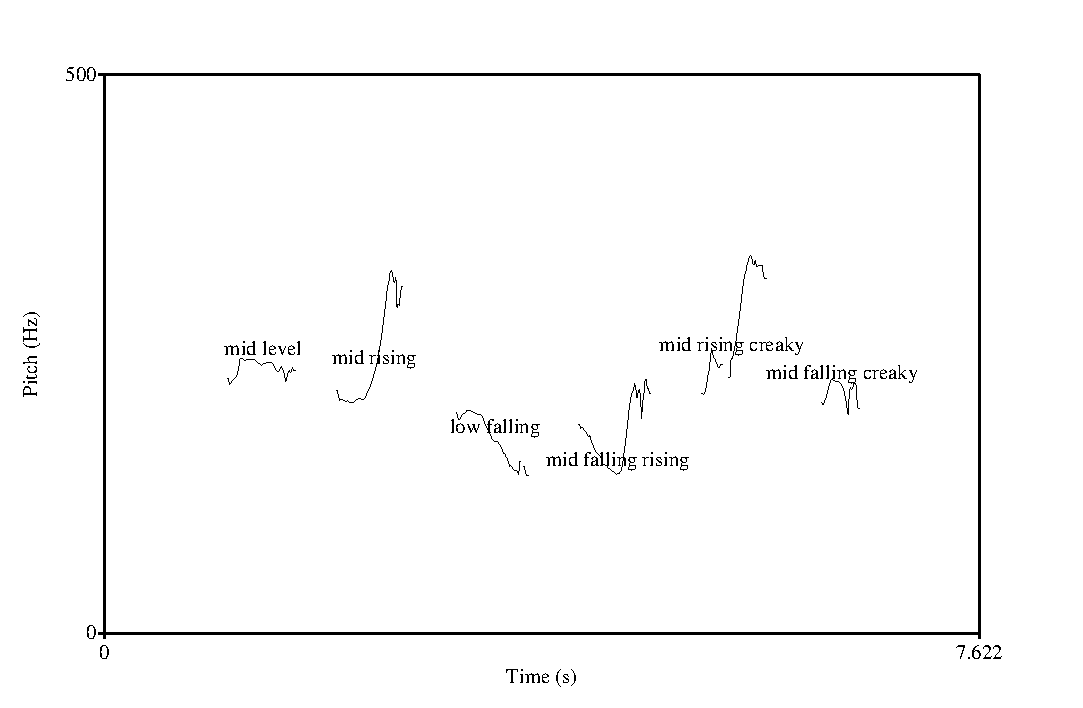
\includegraphics[scale=1.0]{praat.eps} 
\caption{Pitch contours of six Northern Vietnamese tones}
\label{fig:tones}
\end{center}   
\end{figure}

In the Central and Southern Vietnamese varieties, the MFR and MRC tones have reportedly been merged into one tone (Emeneau, 1951) \cite{Emeneau:1951aa}, which could be a natural sequence of these tones being similar in contour coupled with the fact that syllables with the MRC tone occur much less often in the language to begin with. Furthermore, the distribution of tones is constrained by the syllable shape for closed syllables: in closed syllables with voiceless stop codas, only the MR and MFC tones are licensed. The following table shows this constraint applied on closed syllables with voiceless stop codas, compared to open syllables and closed syllables with nasal codas. Because only nasals, voiceless stops, and approximants can appear as codas, Table \ref{tab:table2} presents all possible consonantal coda classes and their associated tone distributions. 

%This constraint in tone distribution motivates the second research question of this study, and will be discussed shortly in subsequent sections.

\begin{table}[H]
  \begin{center}
    \caption{Tone distribution in Vietnamese}
    \label{tab:table2}
      \begin{tabular}{|p{2cm}|p{3cm}|p{3cm}|p{3cm}|p{3cm}}
      \hline
       & Open syllable & Closed syllable with nasal coda & Closed syllable with voiceless stop coda\\\hline
      ML & \checkmark ma & \checkmark man & X \\\hline
     MR & \checkmark  má & \checkmark mán & \checkmark mát \\\hline
      LF & \checkmark mà & \checkmark màn & X \\\hline
     MFR & \checkmark ma?  & \checkmark ma?n & X \\\hline
      MRC & \checkmark mã & \checkmark mãn & X \\\hline
     MFC & \checkmark  ma. & \checkmark ma.n & \checkmark ma.t \\\hline
   
    \end{tabular}
  \end{center}
\end{table}

Having surveyed briefly the characteristics of stress in American English and tone in Vietnamese, let us turn to the next key concept that also serves as one of the central pieces of this paper's theoretical foundations: speech perception.


% Stress-accent differ from nonstress-accent languages such as Japanese, in that pitch accents are not only characterized by a pitch movement but also by other acoustic correlates such as greater duration and loudness 􏰈Beckman, 1986􏰀. (from Spectral balance paper)% Not relevant to my paper.
\subsection{Speech Perception}

Speech perception is the process of mapping of sounds into linguistic representations in the brain (Zsiga, 2013). This process begins with \textit{hearing} where the speech signals are received by the ear and various information such as amplitude, frequency, timing, and so on of the signals is transmitted down the auditory pathway. Speech perception is thought to occur in the auditory cortex, where extracted auditory cues such as the F0, formant transitions, amplitude variations, and so on are matched to a stored linguistic unit \cite{Zsiga:2013aa}. The basilar membrane in the Cochea can perform Fourier-like analysis of the speech signals, specifically, the thin end of this membrane responds to high frequency components in the speech signal and the thick end of the membrane responds to low frequency components in the speech signal. Perception of sounds produced by different individuals is made possible by normalization of raw values so that perception is tuned to relative values, rather than absolute ones. This mechanism would enable us to map sounds produced by male and female speakers as belonging to the same category, despite the discrepancy in absolute terms. A notable feature of speech perception in humans is termed \textit{categorical perception}, which means that humans tend to be good at distinguishing sounds that fall into different phonemic categories in their language as these sounds are contrastive and poor at distinguishing sounds that fall into the same category, even though acoustically these sounds might have different representations. (Liberman, 1957) tested participants' responses to synthesized stimuli of various voiced stops followed by a near-open front unrounded vowel and found that discrimination of the voiced stops along the place of articulation was robust, but discrimination of sounds within the same category was not.  \textit{Categorical perception} was also confirmed cross-linguistically (Abramson and Lisker,1970; Abramson and Lisker, 1973) by studies that looked at different languages' voice onset time (VOT) contrasts and the correlation with perception of the same sounds. The researchers found that the category boundary of VOT differs from language to language. For example, speakers of English have category boundary of 30 ms VOT for `ba' and `pa', thus tokens with VOT of more than 30 ms were perceived to be `pa' and tokens with VOT of less than 30 ms were perceived to be `ba'. For speakers of Spanish whose /b/ sound has a negative VOT, which indicates pre-voicing, and /p/ sound is voiceless unaspirated, the category boundary for `ba' and `pa' was found to be much lower, at 15 ms. For Thai speakers, categorical perception of voicing can be divided into three regions, /b/ would be perceived for VOT less than -20 ms, as Thai has pre-voicing /b/, /p/ would be perceived for VOT between -20 and +40 ms, and aspirated /p/ for VOT above +40 ms \cite{Abramson:1970aa} \cite{Abramson:1973aa}. Another well-known evidence supporting the \textit{categorical perception} notion is Japanese speakers' insensitivity to the contrast between liquid sounds /r/ and /l/, as these sounds are allophones of the same phoneme in Japanese (Goto, 1971; Miyawaki et al., 1975) \cite{Goto:1971aa}.

Speech perceptions studies often try to shed light onto the puzzle that humans are able to map continuous speech stream into discrete segments such as the phonemes. There seems to be a disconnection between the acoustics of speech and how the same information is represented abstractly in phonology. For instance, (Kenstowicz, 1994) remarked that it is difficult to segment waveforms into separate phonemes while discarding information from adjacent phonemes, due to coarticulation. Despite overlapping information in the acoustic signals, humans are able to perceive segments in discrete categories, as some studies have shown through evidence of categorical perception. To explain this curious dilemma, the \textit{Motor Theory} (Liberman et al., 1967) posits that perception is more closely related to articulatory gestures than to acoustics. The argument for this arises from the fact that the same /d/ phoneme could be perceived out of completely different acoustic signals, specifically, /d/ could be perceived from two different F2 formant transition patterns in /di/ and /du/, where the transition goes down in the former and up in the latter. 

In the domain of prosody, native speakers of tone languages were found to have categorical perception of tones whereas naive listeners do not (Shen and Froud, 2016). Previous studies have also shown that native speakers of a stress language may have a smaller perceptual space of tones than that of native speakers of a tone language as they took longer to judge if two tones were different, suggesting that on average the tones were less distinct for the former group (Huang, 2001) \cite{Huang:2001aa}. Notably, several studies on stress perception by speakers of different L1 stress languages showed that speakers of L1 fixed-stress languages such as Arabic, Turkish, and French performed worse than speakers of unpredictable stress languages such as Spanish and speakers of L1 without stress such as Japanese, Korean, Chinese in stress perception tasks in English. Speakers of L1 with fixed stress were thought to lack a metalinguistic representation of contrastive stress in their L1 phonological representation and therefore were impaired in stress perception tasks, which is congruent with the \textit{categorical perception} notion (Dupoux, Sebastian-Galles, Navarrete, and Peperkamp, 2008) \cite{Dupoux:2008aa}. Chinese speakers showed greater discrimination peakedness compared to English speakers in intonation perception, explained by the interaction of F0 in lexical tones and pitch contours of intonation in Chinese that is absent in English (Liu and Rodriguez, 2012). Interaction of lexical tone on prosody was shown via another study which found that Chinese speakers have a harder time identifying a rising intonation associated with questions when the final word in the sentence has a rising tone, compared to a final falling tone (Yuan, 2011). Similarly, (Ma et al., 2011) found that perception of intonation in questions and statements of Cantonese depends on the F0 of the final syllable. Besides F0, amplitude of the final word was also found to be a secondary cue to question or statement intonation perception (Morrow, 2013). 

From these previous studies and conclusions, it could be expected that perception of stress by native speakers of a tone language would be significantly influenced by the L1's prosodic characteristics. The next section discusses the prosodic characteristics of stress and tone languages in order to provide more background towards forming the research questions.


\subsubsection{Towards forming the research questions}

What exactly are prosodic characteristics' differences between a stress versus a tone language? It turns out that the demarcation between a stress and a tone language is not as clear as what one would expect. English, though classified as a stress-timed language, does employ lexical pitch contrast akin to a tone language's technique in a limited number of cases, such as in the case of ‘uh-huh', which can mean ‘yes’ or ‘no’, depending on the pitch patterns (Yip, 2002) \cite{Yip:2002aa}. 
% Articular model (Halle) influential in phonological theory -- maybe not aplicable to me.

Evaluating from the acoustic correlates of stress and tone described above suggests that acoustic correlates for stress and tones overlap in pitch and duration, thus it might be the case that learners of English whose native language is a tone language would rely on F0 and syllable length as primary cues to identify stress. On the other hand, studies have argued that English speakers have a tendency to perceive lexical stress using segmental cues, such as vowel reduction, rather than suprasegmental.
Therefore, even though pitch might be the most important correlate of stress in English, according to the literature reviewed in \ref{American English as a stress-timed language},  and also used by Vietnamese speakers as cue in perception, the way pitch is correlated to stress position and understood by these two groups is not the same. 
%it is not always reliable because pitch is easily confounded with phrase and sentence level intonation.
 For example, Ladefoged has demonstrated in his classic textbook for Phonetics \textit{A Course in Phonetics} the different intonation patterns of the same word `Amelia', where the second stressed syllable receives a high pitch in a statement sentence and a low pitch in a yes/no question, because the intonation for a statement is H* L L\% and the intonation for a yes/no question is L* H H\% (Ladefoged, 1993) \cite{Ladefoged:1993aa}. This phenomenon was measured empirically in Ou (2010) and replicated here in Table \ref{tab:table3} and Table \ref{tab:table4} \cite{Ou:2010aa}.

\begin{table}[!h]
  \begin{center}
      \caption{Phonetic measures of stressed and unstressed syllables of nonce words in the falling intonation}
\begin{tabular}{lllll}
    \label{tab:table3}
              & \multicolumn{2}{l}{FERcept} & \multicolumn{2}{l}{ferCEPT}  \\ \hline
 Syllable & FER          & cept          &   fer          &      CEPT        \\ \hline
F0 average (Hz) & 281          & 141          &   147           &      233         \\ \hline
Intensity (dB)    & 79           & 69          &      70        &         74    \\ \hline
Duration (ms)     & 118          & 98        &       55      &      133
\end{tabular}
\end{center}
\end{table}

\begin{table}[!h]
  \begin{center}
      \caption{Phonetic measures of stressed and unstressed syllables of nonce words in the rising intonation}
\begin{tabular}{lllll}
    \label{tab:table4}
              & \multicolumn{2}{l}{FERcept} & \multicolumn{2}{l}{ferCEPT}  \\ \hline
 Syllable & FER          & cept          &   fer          &      CEPT        \\ \hline
F0 average (Hz) & 151          & 256          &   153           &      177         \\ \hline
Intensity (dB)    & 65           & 73         &      63        &         69    \\ \hline
Duration (ms)     & 116          & 119        &       63      &      69
\end{tabular}
\end{center}
\end{table}

Ou (2010) explained that in the falling intonation of a statement context, the phonetic measures pattern as expected, in other words, all three phonetic measures of the stressed syllable were higher than those of the unstressed syllable. In the rising intonation of a yes/no question context, however, this pattern no longer holds. In fact, all three measures of the stressed syllable in the word-initial position were lower than those of the unstressed syllable. Ou (2010) explained that in the rising intonation condition, `when the second syllable is stressed, it has a low rising pitch contour, when the second syllable is unstressed, it has a high rising pitch contour' \cite{Ou:2010aa}. That is because the word with initial stress would have a rising contour that starts earlier than the word with final stress. Ou (2010) manipulated the context where the stressed syllable occurs, and predicted that speakers of a tone language would have difficulty in perceiving the stress location in a low rising tonal contour context such as that of a yes/no question ( L* H H\% ), as English stressed syllable actually receives a low tone then \cite{Ou:2010aa}. This study motivated the first research question and the pilot study reported in this paper.

Nguyen and Ingram (2005) \cite{Nguyen:2005aa} confirmed that Vietnamese speakers were able to differentiate stress contrasts in English as well as the native speaker group did in production, because Vietnamese speakers are used to using pitch and intensity as cue in tonal production. This study lent support for the hypothesis that speakers of languages whose acoustic cues match those of the target language would employ those cues in perception and/or production of the L1. Factors such as duration and vowel reduction, non-native elements of prosody perception, were not readily employed when the learners tried to identify stress in English, nor were they successfully replicated in production (Nguyen and Ingram, 2005) \cite{Nguyen:2005aa}. From the perception side, Nguyen (2017) specifically looked at tonal assignment as a result of stress perception. The study concluded that an English syllable could be perceived to carry a certain Vietnamese tone, depending on the syllable structure and relative F0 levels. This study's method centered around asking participants to transcribe target syllables that they have heard into the closest equivalent in Vietnamese using Vietnamese orthography. This method would inevitably be able to elicit the participants' mapping of English word stress with Vietnamese tones because Vietnamese orthography mandates tone assignment for each written syllable. The target syllables are bisyllabic real words such as \textit{present - verb} and \textit{present - noun}, and compounds such as \textit{silver fish - fish made of silver} and \textit{silver fish - not a golden fish} and \textit{silverfish - a type of insect}. The result of this study showed that Vietnamese native speakers used relative F0 as cue for stress to tone mapping (Nguyen, 2017) \cite{Nguyen:2017aa}. Interestingly, the prediction that English syllables ending in obstruents will be perceived as having the rising tone (MR) if stressed and having the drop tone (MFC) if unstressed was only partially born out. Syllables ending in obstruents that are unstressed were still perceived to carry the rising tone (MR) by many speakers. The study also analyzed different responses of speakers due to dialectal differences with respect to tone assignment of stressed syllables ending in a sonorant, where Southern speakers preferred to assign the MR tone and speakers of the Central and Northern dialect preferred to assign the ML tone. In a similar vein, the topic of tonal assignment to stress in foreign words borrowed into Vietnamese could be inferred from a report on phonological adaptation of French loanwords in Vietnamese by Scholvin and Meinschaefer (2018) \cite{Scholvin:2018aa}, whose data seemed to show that final syllables in a bisyllabic loanword are often assigned a level or rising tone, rather than a low tone, which seems to be congruent with the fact that French words are stressed on the last syllables and Vietnamese level and rising tones have a tendency to be associated with stressed syllables.

Not many studies have been done to examine how Vietnamese learners acquire English word stress, especially from the perception side. (Nguyen, 2005) reported findings on the transfer of tonal correlates in Vietnamese speakers' production of English words and found that while Vietnamese learners' production of English word stress mimicked F0 and intensity contrasts between stressed and unstressed syllables, the production of beginners fell short of replicating vowel duration and quality contrasts accurately, namely, the beginning learners had issues with reducing vowels to schwas in unstressed syllables.

\section{Research Questions and Hypotheses}
\label{RQ}
Based on the prior literature, particularly motivated by the results found in Ou (2010) and Nguyen (2017), this study proposes the following three research questions.
\begin{enumerate}
  \item Research question 1: Do L1 Vietnamese L2 English speakers have more difficulty than American English native speakers in identifying stress location in yes/no question context where the stressed syllable does not necessarily have higher F0 than the other syllable(s)?
   \item Research question 2: Would difficulty in identifying the stress location in the yes/no question context manifest in a delayed reaction to the stimuli in the L2 English group?
  \item Research question 3: Does early arrival bestow an advantage on L2 speakers? Would L2 speakers who moved to the United States at a young age perform better at the stress matching task?
\end{enumerate}



Given previous studies such as Ou (2010) and Nguyen (2017), the predictions to the aforementioned research questions are as follows.
\begin{enumerate}
  \item Prediction 1: Vietnamese native speakers would have difficulty perceiving lexical stress location in contexts of a yes/no question when the stress is not word-final because of L1’s prominence of pitch as a cue for tone perception and of pitch's unreliability as indicator of stress location in this case for the L1 Vietnamese speakers.
   \item Prediction 2: Yes, difficulty in identifying the stress location in the yes/no question context would manifest in a delayed reaction to the stimuli and slower response from the L2 English participants.
   \item Prediction 3: Early arrival might create an advantage for L2 learners and early arrivers would perform better than later arrivers at the stress matching task.
\end{enumerate}

\section{Methodology}

% Participants
\subsection{Participants}

The target participants for this study are adult L1 Vietnamese L2 English speakers with normal hearing ability. The control group is made up of adult native American English speakers. The recruitment process was done both via Amazon Mechanical Turk and offline and all study procedures were conducted with approval of the Institutional Review Board at the University of Illinois at Urbana Champaign. Forty-six participants participated in the study, representing two groups: (1) native American English speakers (n=26, age range = 18-69, average age =  37.88, median age = 34.5) and (2) native Vietnamese speakers who currently reside in the United States (n = 20, age range = 19-39, average age = 30.45). All participants reported no hearing difficulties. Each participant signed an informed consent form prior to taking part in the study and all received a compensation of 10 dollars for the time spent on the survey. The participants submitted responses to the survey at a distance from the researcher \footnote{because of restrictions on in-person research due to the ongoing coronavirus pandemic}. In order to verify that the participants are indeed native speakers of the respective languages, cloze tests in English and Vietnamese were included as a screening procedure. Performance on the fillers of the main test was also used as part of criteria to screen Amazon Turk workers. If the percentage score of the cloze test and fillers was less than 80 percent, the worker's response was discarded.The English cloze test consists of 50 fill in the blank questions and the Vietnamese cloze test consists of 14 fill in the blank questions. American English native speakers spent on average 16 minutes on the English cloze test while the Vietnamese speakers spent on average 25 minutes on the English cloze test. All participants in the experimental group scored at least 90 percent on the Vietnamese cloze test, in other words, no one got more than one wrong for this screening test. Results of the English cloze test from the two groups will be discussed in the Discussion section.
 
Both groups answered a questionnaire about their language background, hearing ability, and demographics before the study began. 

All Vietnamese speakers were born in Vietnam (in Hai Phong (n = 1), Ho Chi Minh City (n = 10), Ha Noi (n = 8), Dong Nai (n = 1), or Hue (n = 1)). Nine participants reported to be native speakers of the northern dialect, 10 participants reported to be native speakers of the southern dialect, and 1 participant reported to be native speaker of the central dialect. On average, Vietnamese speakers began learning English from 8.1 years old (median = 8), with one starting the earliest from 4 years old and one starting the latest from 15 years old. The length of formal instruction as well as experience in using English for the Vietnamese native speakers is about 22 years on average, with a range between 14 to 32 years. On average, they moved to the United States at 20.75 years of age (median = 18), the youngest at 11 and the oldest at 37. The shortest duration of residence in the United States is 2.08 years and the longest duration of residence is 19.08 years. On average, the experimental group has been living in the United States for 9.73 years (median = 11). They reported knowledge of other languages other than English, including Spanish, French, Mandarin Chinese (n = 6), French (n = 5), Spanish (n = 1), Japanese (n = 1), Portuguese (n = 1), and Korean (n = 1).

The American English native speakers were all born in the United States (California (n = 8), Illinois (n = 3), Ohio (n = 2), Florida (n = 2), Georgia (n = 1), Michigan (n = 3), North Carolina (n = 2), New York (n = 2), New Hampshire (n = 1), Texas (n = 1), Washington State (n = 1). They reported knowledge of other languages other than English, including Mandarin Chinese (n = 3), Spanish (n = 11), French (n = 2), Japanese (n = 3), Bisaya (n = 1), Cantonese (n = 2). 11 participants reported to be monolinguals.

% Materials
\subsection{Materials}

To avoid lexical retrieval and memorization effect, nonce words were created as stimuli for this experiment. In cases where it was difficult for a brand new nonce word to be created, a real word was used if it was deemed to be rare or is a proper name or a loanword. In most cases, the stimuli ended up to be proper names. In order to choose the nonce words, an interactive search in the CMU Pronouncing Dictionary for US English corpus provided in the NLTK toolkit was performed. The target stimuli included bisyllabic and trisyllabic words, thus the first set of queried results consists of bisyllabic words and the second set of queried results consists of trisyllabic words. The two sets consist of words with ambiguous stress patterns, in other words, the first set returns bisyllabic words where both word-initial and word-final stress are possible (Appendix \ref{appendix:a}) and the second set returns trisyllabic words where word-initial, word-medial, and word-final stress are possible (Appendix \ref{appendix:b}). For the majority of cases, the stimuli were directly taken from the returned set of words from the query, with some modification to ensure that vowel reduction is unlikely during the recording of these words with different stress patterns. Words that are also proper names were also used directly without modification, for example \textit{taebak}. Because the search for trisyllabic words with ambiguous stress positions returned only three results, trisyllabic words that may be proper names were used and the different stress positions applied on them. All of the stimuli were double checked by a native speaker to make sure that no real common words appeared among the stimuli, and that the different stress positions within each stimulus are possible in English.

Test sentences were created to satisfy 4 test conditions for bisyllabic words, due to the crossing of 2 factors: the stress position (2 levels: word-initial and word-final) with the intonation context type (2 levels: statement sentence and yes/no question sentence), as shown in Table \ref{tab:table5} and 6 test conditions for trisyllabic words, due to the crossing of 2 factors: the stress position (3 levels: word-initial, word-medial, and word-final) with the intonation context type (2 levels: statement sentence and yes/no question sentence), as shown in Table \ref{tab:table6}. The sentences were used as an aid for the recording procedure, in order to elicit a natural statement and question intonation from the English speaker. The sentences are similar in structure and the stimuli appear in all test sentences as nouns or proper names, in order to control for part of speech and bias related to part of speech due to English paradigmatic characteristics of stress. Based on the hypothesis posited in Section \nameref{RQ}, L1 Vietnamese L2 English speakers are predicted to have more difficulty and lower performance than the control group in identifying stress location of the conditions marked with the double asterisks. The tables below show the stimuli created for the recording step. These stimuli were later extracted from the originally recorded sentences so that only the words remain for the participants to evaluate.

\begin{table}[H]
  \begin{center}
    \caption{2 X 2 design for bisyllabic words. A tokens set example}
    \label{tab:table5}
      \begin{tabular}{|p{5cm}|p{4cm}|p{4cm}|p{4cm}}
      \hline
       & Stress initial & Stress final \\
      \hline
      Word in a statement sentence & He is a GAUbert. & He is a gauBERT. \\
      \hline
      Word in a yes/no question sentence & **Is he a GAUbert? & Is he a gauBERT? \\
      \hline
    \end{tabular}
  \end{center}
\end{table}


\begin{table}[H]
  \begin{center}
    \caption{2 X 3 design for trisyllabic words. A tokens set example}
    \label{tab:table6}
      \begin{tabular}{|p{4cm}|p{3cm}|p{3cm}|p{3cm}|p{3cm}}
      \hline
       & Stress initial & Stress middle & Stress final \\
      \hline
      Word in a statement sentence & That is a CAseybeer. & That is a caSEYbeer. & That is a caseyBEER. \\
      \hline
      Word in a yes/no question sentence & **Is that a CAseybeer? & **Is that a caSEYbeer? & Is that a caseyBEER? \\
      \hline
    \end{tabular}
  \end{center}
\end{table}

Seventeen bisyllabic words were chosen for recording, resulting in 102 sound files (17 x 6, 2 stimuli uttered in isolation in two stress patterns, 2x2 additional stimuli based on the crossed conditions) and 19 trisyllabic words were chosen for recording, resulting in 171 sound files (19 x 9, 3 stimuli uttered in isolation in three stress patterns, 3x2 additional stimuli based on the crossed conditions) (see Appendix \ref{testitems}). 19 word pairs were created as fillers. The fillers were mainly word pairs that differ in other dimensions such as segmental contrasts, vowel length, word length, and so on. A mix of real and nonce words could be found in the fillers set. A sentence containing one of the words in the pair was created for recording. The fillers were also used to screen workers in Amazon Mechanical Turk. Table \ref{tab:table7} below shows a few examples of fillers and the word pairs' differences. 16 real words with stress location differences were recorded for a transcription task. \footnote{These data will be used for another project and not discussed in this paper}


\begin{table}[H]
  \begin{center}
    \caption{Filler examples}
    \label{tab:table7}
      \begin{tabular}{|p{5cm}|p{4cm}|p{4cm}|p{4cm}}
      \hline
        Filler & Type of difference \\
      \hline
     close /z/ and close /s/ & voicing \\
      \hline
      repair and repaired & presence of the past morpheme  \\
            \hline
      tirade and tirades & presence of the plural morpheme \\
                  \hline
      fim and feam & vowel length \\
                        \hline
      wander and wonder & vowel quality \\
      \hline
    \end{tabular}
  \end{center}
\end{table}

The recording was done by a graduate student of Linguistics who is an American English native speaker, using Praat at sampling frequency 44,100 Hz. Reviewing of the recording shows that it was difficult for the speaker to control for vowel reduction in the recording of trisyllabic words. Consequently, many trisyllabic words that were recorded ended up not being used in the study. In total, 16 bisyllabic words and 6 trisyllabic words were chosen for the study. The fillers set was supplemented by a previously recorded fillers set that was used for the pilot study, totalling 38 fillers (see appendix \ref{fillers} for all the fillers). 

All words were manually labelled and extracted from the original recording using Praat for further acoustic analysis, totalling 264 sound files. High pass filtering was applied when applicable to remove noise from the recording. The sound clips were concatenated for each stimulus, with a 1-second silence period in between two words or in between three words and copied to create a new sound clip with the sounds repeated three times, and each repetition was separated by a 2-second silence period. Stimuli were embedded in a Qualtrics survey in autoplay mode, so that participants would not have control over when the sounds are played to them. The example below demonstrates how GAUbert and ROseemund appeared in the test instrument. The order of the first round of stimuli does not correspond to the stress order in the words; in other words, sometimes, the word with syllable-initial stress was played first, sometimes the other way around. The order of the stimuli's presentation was randomized.

\begin{description}
  \item \textit{Audio playing: GAUbert - pause - gauBERT - pause - GAUbert - pause - gauBERT  - pause - GAUbert - pause - gauBERT }
  \item \textit{Audio playing: GAUbert (question intonation).} 
  \item Question: The sentence being played contains one of the sounds you've heard previously. Which one is it? Answer choices: FIRST SOUND, SECOND SOUND
  \item \textit{Audio playing: ROseemund - pause - roSEEmund - pause - roseeMUND - pause - ROseemund - pause - roSEEmund - pause - roseeMUND - pause - ROseemund - pause - roSEEmund - pause - roseeMUND}
    \item \textit{Audio playing: ROseemund (statement intonation).} 
  \item Question: The sentence being played contains one of the sounds you've heard previously. Which one is it? Answer choices: FIRST SOUND, SECOND SOUND, THIRD SOUND

\end{description}

The test instrument was built from 4 blocks, where each block contains 5 or 6 stimuli (4 stimuli from the bisyllabic words, corresponding to 4 conditions and either one or two trisyllabic words) and 10 or 9 fillers (see Appendix \ref{full}). Each test block therefore contains 15 stimuli. The stimuli were randomized within each block. Six test lists were created using a Latin square design, so that each participant only sees one stimulus from each tokens set. The test lists were distributed relatively proportionally among the participants. Each test list collected from between 3 to 6 responses.

After finishing the speech perception task, L1 Vietnamese L2 English participants were asked to transcribe 16 real words using Vietnamese orthography, specifying in details the tone marks and diacritics\footnote{These data will be used for another project and not discussed in this paper}.

\subsection{Procedure}

The participants answered the test online via a web link issued by Qualtrics\footnote{The full tests are located at https://illinoislas.qualtrics.com/jfe/form/SV_3lztPSumrMhCbOd (experimental group test) https://illinoislas.qualtrics.com/jfe/form/SV_54kNUrkuoC3IrqJ (control group test). These are only two test lists out of twelve test lists that were constructed}. Six test lists were available for the L1 English speakers and six other test lists were available for the L1 Vietnamese speakers. Besides the background questionnaire and the screening cloze test mentioned in the previous section, the test instrument includes two practice questions, 60 forced choice speech perception questions, and 16 transcription questions that only the experimental group completed\footnote{These data will be used for another project and not discussed in this paper}.

In the main test, the participants were instructed to listen to the stimuli in groups of two or three and take note of the difference(s) among the items. The participants completed two practice questions before the actual test began. The audio of the stimuli was repeated three times, for example, `GAUbert - pause - gauBERT - pause - GAUbert - pause - gauBERT  - pause - GAUbert - pause - gauBERT'. The participants did not have control over the audio. The audio played automatically when they moved through the survey page by page. After the  audio finished playing, the participants would click `Next' to go to the forced choice perception task. In this task, the participants listened to a word containing one of the stimuli previously uttered as a single word, but uttered with a statement or a question intonation. For example, `GAUbert (question intonation)'. This stimulus was also repeated three times. The participants then answered if the word just uttered was the first or second word (or third word if the question concerns a trisyllabic word) of the words that they have just heard previously. Once the participants answered and moved onto the next question, they were not able to return and edit their answer. The time participants spent on each question, the reaction time, and the number of clicks in response to the stimuli were recorded.

The transcription task consisted of an audio of a word, repeated three times to the participants. Only Vietnamese speakers completed this task. The speakers were instructed to transcribe the words they heard using Vietnamese orthography, specifying tone markers and diacritics.

\subsection{Acoustic statistics of the stimuli}

All stimuli used in the test were natural recordings. Upon obtaining the recordings of the stimuli, some acoustic statistics were extracted from the speech samples (see Table \ref{tab:tablestressedsyl}). As this study concerns the impact on F0 on stress perception, the average F0 values of all stressed syllables were calculated for each stimulus. The procedure was done using the Praat software. The stressed syllables were manually segmented and labeled in a TextGrid, and a script was written to extract these stressed syllables as well as query out F0 values from three equally spaced time points. The table below presents the F0 values of stressed syllables in the bisyllabic stimuli and the stressed syllable's duration. Where the stressed syllable was too short, it was not always possible to obtain three F0 values from the speech signal. The word-intial stress was coded as 10, the word-final stress was coded as 01, _d was a code for the statement intonation, and q_ was a code for the question intonation. For many of these cases, the F0 on the stressed syllable in the word initial position, question intonation was lowered than the F0 in the stressed syllable in the word-initial position, statement intonation. However, it is not always the case, we might need to look at the relative change within a word to see how the F0 in the word-initial position compares between questions and statements. 

\begin{table}[H]
    \label{tab:tablestressedsyl}
\begin{tabular}{|l|r|l|r|l|r|} 
\hline
Stimuli         & \multicolumn{1}{l|}{Duration} & F0 at A                           & \multicolumn{1}{l|}{F0 at B}            & F0 at C                       & \multicolumn{1}{l|}{Average F0}  \\ 
\hline
10\_gaubert\_d~ & 0.207                         & \multicolumn{1}{r|}{196.750} & \multicolumn{1}{l|}{164.05}        & \multicolumn{1}{r|}{156.690} & 176.720                          \\ 
\hline
10\_gaubert\_q~ & 0.209                         & \multicolumn{1}{r|}{155.250} & 150.930                            & \multicolumn{1}{r|}{159.070} & 155.083                          \\ 
\hline
01\_gaubert\_d~ & 0.244                         & \multicolumn{1}{r|}{172.550} & 133.340                            & --undefined--                & 152.945                          \\ 
\hline
01\_gaubert\_q~ & 0.234                         & \multicolumn{1}{r|}{161.630} & 184.980                            & --undefined--                & 173.305                          \\ 
\hline
10\_pokgrom\_d~ & 0.182                         & --undefined--                & 219.460                            & --undefined--                & 219.460                          \\ 
\hline
10\_pokgrom\_q~ & 0.277                         & --undefined--                & 212.760                            & --undefined--                & 212.760                          \\ 
\hline
01\_pokgrom\_d~ & 0.562                         & 191.25                       & 147.970                            & --undefined--                & 147.970                          \\ 
\hline
01\_pokgrom\_q~ & 0.320                         & \multicolumn{1}{r|}{171.020} & 192.450                            & --undefined--                & 181.735                          \\ 
\hline
10\_taebak\_d~  & 0.248                         & --undefined--                & 207.160                            & 147.92                       & 207.160                          \\ 
\hline
10\_taebak\_q~  & 0.200                         & --undefined--                & 160.980                            & \multicolumn{1}{r|}{169.860} & 165.420                          \\ 
\hline
01\_taebak\_d~  & 0.377                         & 170.69                       & \multicolumn{1}{l|}{--undefined--} & --undefined--                & \multicolumn{1}{l|}{170.69}      \\ 
\hline
01\_taebak\_q~  & 0.412                         & --undefined--                & \multicolumn{1}{l|}{289.03}        & --undefined--                & \multicolumn{1}{l|}{289.03}      \\ 
\hline
10\_saevir\_d~  & 0.197                         & 201.65                       & 176.880                            & 164.95                       & 176.880                          \\ 
\hline
10\_saevir\_q~  & 0.170                         & \multicolumn{1}{r|}{186.520} & 175.240                            & \multicolumn{1}{r|}{178.390} & 180.050                          \\ 
\hline
01\_saevir\_d~  & 0.364                         & \multicolumn{1}{r|}{185.180} & \multicolumn{1}{l|}{--undefined--} & --undefined--                & 185.180                          \\ 
\hline
01\_saevir\_q~  & 0.246                         & \multicolumn{1}{r|}{178.900} & \multicolumn{1}{l|}{180.91}        & --undefined--                & 178.900                          \\ 
\hline
10\_moray\_d~   & 0.277                         & \multicolumn{1}{r|}{173.730} & 165.100                            & 166.05                       & 169.415                          \\ 
\hline
10\_moray\_q~   & 0.192                         & \multicolumn{1}{r|}{201.520} & 183.190                            & \multicolumn{1}{r|}{169.520} & 184.743                          \\ 
\hline
01\_moray\_q~   & 0.303                         & \multicolumn{1}{r|}{170.890} & 206.190                            & \multicolumn{1}{r|}{289.800} & 222.293                          \\ 
\hline
01\_moray\_d~   & 0.437                         & \multicolumn{1}{r|}{193.110} & \multicolumn{1}{l|}{--undefined--} & --undefined--                & 193.110                          \\ 
\hline
10\_moshee\_d~  & 0.299                         & \multicolumn{1}{r|}{167.800} & \multicolumn{1}{l|}{180.07}        & 178.32                       & 167.800                          \\ 
\hline
10\_moshee\_q~  & 0.287                         & \multicolumn{1}{r|}{174.740} & 226.750                            & --undefined--                & 200.745                          \\ 
\hline
01\_moshee\_d~  & 0.536                         & \multicolumn{1}{r|}{158.200} & 167.630                            & --undefined--                & 162.915                          \\ 
\hline
01\_moshee\_q~  & 0.349                         & --undefined--                & 196.160                            & 362.45                       & 196.160                          \\ 
\hline
10\_panshee\_d~ & 0.286                         & --undefined--                & 212.400                            & \multicolumn{1}{r|}{186.450} & 199.425                          \\ 
\hline
10\_panshee\_q~ & 0.265                         & --undefined--                & 178.590                            & \multicolumn{1}{r|}{201.240} & 189.915                          \\ 
\hline
01\_panshee\_d~ & 0.473                         & --undefined--                & 168.530                            & --undefined--                & 168.530                          \\ 
\hline
01\_panshee\_q~ & 0.331                         & --undefined--                & 321.480                            & --undefined--                & 321.480                          \\ 
\hline
10\_tanvo\_d~   & 0.328                         & --undefined--                & 201.870                            & 165.93                       & 201.870                          \\ 
\hline
10\_tanvo\_q~   & 0.314                         & --undefined--                & 182.280                            & \multicolumn{1}{r|}{169.440} & 175.860                          \\ 
\hline
01\_tanvo\_d~   & 0.377                         & 201.40                       & 153.980                            & --undefined--                & 153.980                          \\ 
\hline
01\_tanvo\_q~   & 0.341                         & \multicolumn{1}{r|}{166.460} & 206.960                            & --undefined--                & 186.710                          \\ 
\hline
10\_oblak\_d~   & 0.212                         & --undefined--                & 175.130                            & 186.90                       & 175.130                          \\ 
\hline
10\_oblak\_q~   & 0.174                         & 172.03                       & 163.410                            & \multicolumn{1}{r|}{173.940} & 168.675                          \\ 
\hline
01\_oblak\_d~   & 0.480                         & \multicolumn{1}{r|}{185.490} & \multicolumn{1}{l|}{--undefined--} & --undefined--                & 185.490                          \\ 
\hline
01\_oblak\_q~   & 0.421                         & \multicolumn{1}{r|}{173.280} & \multicolumn{1}{l|}{329.17}        & --undefined--                & 173.280                          \\ 
\hline
10\_anna\_d~    & 0.294                         & --undefined--                & 197.430                            & 158.41                       & 197.430                          \\ 
\hline
10\_anna\_q~    & 0.180                         & 146.71                       & 175.500                            & \multicolumn{1}{r|}{187.730} & 181.615                          \\ 
\hline
01\_anna\_d~    & 0.313                         & \multicolumn{1}{r|}{191.370} & \multicolumn{1}{l|}{--undefined--} & \multicolumn{1}{r|}{182.470} & 186.920                          \\ 
\hline
01\_anna\_q~    & 0.318                         & \multicolumn{1}{r|}{174.740} & \multicolumn{1}{l|}{212.45}        & --undefined--                & 174.740                          \\ 
\hline
10\_danbah\_d~  & 0.300                         & --undefined--                & 187.580                            & 159.58                       & 187.580                          \\ 
\hline
10\_danbah\_q~  & 0.272                         & 186.04                       & 161.910                            & --undefined--                & 161.910                          \\ 
\hline
01\_danbah\_d~  & 0.372                         & \multicolumn{1}{r|}{208.770} & \multicolumn{1}{l|}{--undefined--} & --undefined--                & 208.770                          \\ 
\hline
01\_danbah\_q~  & 0.296                         & --undefined--                & \multicolumn{1}{l|}{248.64}        & --undefined--                & \multicolumn{1}{l|}{248.64}      \\ 

\end{tabular}
\end{table}

\begin{table}[H]
    \label{tab:tablestressedsyl}
\begin{tabular}{|l|r|l|r|l|r|} 
\hline
Stimuli         & \multicolumn{1}{l|}{Duration} & F0 at A                           & \multicolumn{1}{l|}{F0 at B}            & F0 at C                       & \multicolumn{1}{l|}{Average F0}  \\ 
\hline
10\_bennet\_d~  & \multicolumn{1}{l|}{0.213}    & \multicolumn{1}{r|}{175.140} & \multicolumn{1}{l|}{--undefined--} & \multicolumn{1}{r|}{188.810} & 181.975                          \\ 
\hline
10\_bennet\_q~  & 0.218                         & \multicolumn{1}{r|}{190.330} & \multicolumn{1}{l|}{210.04}        & \multicolumn{1}{r|}{187.790} & 189.060                          \\ 
\hline
01\_bennet\_d~  & 0.283                         & \multicolumn{1}{r|}{182.690} & 175.760                            & --undefined--                & 179.225                          \\ 
\hline
01\_bennet\_q~  & 0.326                         & \multicolumn{1}{r|}{171.580} & 231.100                            & --undefined--                & 201.340                          \\ 
\hline
10\_miro\_d~    & 0.257                         & \multicolumn{1}{r|}{199.540} & 180.540                            & 158.34                       & 190.040                          \\ 
\hline
10\_miro\_q~    & 0.254                         & \multicolumn{1}{r|}{184.330} & 184.350                            & \multicolumn{1}{r|}{218.470} & 195.717                          \\ 
\hline
01\_miro\_d~    & 0.376                         & \multicolumn{1}{r|}{204.740} & 156.620                            & --undefined--                & 180.680                          \\ 
\hline
01\_miro\_q~    & 0.367                         & \multicolumn{1}{r|}{174.120} & 189.200                            & 305.17                       & 181.660                          \\ 
\hline
10\_zaabir\_d~  & 0.335                         & \multicolumn{1}{r|}{177.680} & \multicolumn{1}{l|}{--undefined--} & \multicolumn{1}{r|}{184.330} & 181.005                          \\ 
\hline
10\_zaabir\_q~  & 0.314                         & --undefined--                & \multicolumn{1}{l|}{162.37}        & \multicolumn{1}{r|}{188.840} & 188.840                          \\ 
\hline
01\_zaabir\_d~  & 0.369                         & 218.92                       & 153.370                            & \multicolumn{1}{r|}{172.320} & 162.845                          \\ 
\hline
01\_zaabir\_q~  & 0.379                         & --undefined--                & 196.400                            & --undefined--                & 196.400                          \\ 
\hline
10\_kantar\_d~  & 0.351                         & --undefined--                & 187.430                            & --undefined--                & 187.430                          \\ 
\hline
10\_kantar\_q~  & 0.322                         & --undefined--                & 171.280                            & 173.35                       & 171.280                          \\ 
\hline
01\_kantar\_d~  & 0.440                         & --undefined--                & 163.130                            & \multicolumn{1}{r|}{172.130} & 167.630                          \\ 
\hline
01\_kantar\_q~  & 0.396                         & --undefined--                & 183.590                            & \multicolumn{1}{r|}{318.560} & 251.075                          \\ 
\hline
10\_peenan\_d~  & 0.308                         & --undefined--                & 243.630                            & \multicolumn{1}{r|}{194.860} & 219.245                          \\ 
\hline
10\_peenan\_q~  & 0.234                         & --undefined--                & 201.850                            & \multicolumn{1}{r|}{206.360} & 204.105                          \\ 
\hline
01\_peenan\_d~  & 0.396                         & 204.47                       & 171.300                            & \multicolumn{1}{r|}{167.410} & 169.355                          \\ 
\hline
01\_peenan\_q   & 0.356                         & \multicolumn{1}{r|}{177.810} & 264.220                            & \multicolumn{1}{r|}{295.960} & 245.997                          \\
\hline
\end{tabular}
\end{table}
 
\section{Results}

\subsection{Pilot study result}

%Feedback from Tania: --- REMEMBER TO ADD THIS
% if you are going to report such standardized test scores, you should explain what they mean (what the scale is). 
% mentioned that I have separated the two tests

Prior to conducting this full-scale study, a small pilot study was conducted with six participants. The control group was recruited via Amazon Mechanical Turk and the experimental group was recruited offline. The pilot experimental group's age range is 18 to 34: one participant is 18-24 and two participants are 25-34 of age. They have all started learning English between primary and middle school: at 8, 10, and 11 years old. None of them reported having lived in the United States \footnote{As this was a pilot study, we weren't adamant about finding L2 speakers who reside in the United States. However, this was a requirement in the full study}. They all know a third language (Japanese) with two participants reporting an intermediate level. Two participants reported standardized English test scores, in TOEFL (99), IELTS (7), and TOEIC (955). The control group's age range is 35 to 74, with two participants reporting 35 to 44 age range and the other participant reporting 65 to 74 age range. None of them has had knowledge of another language other than English. The participants responded to the test online via a web link issued by Surveymonkey\footnote{The full tests are located at https://www.surveymonkey.com/r/JQQCY92 (experimental group pilot test) https://www.surveymonkey.com/r/Q688VWJ (control group pilot test)}. Besides the background questionnaire, the test instrument includes one practice question, 80 forced choice speech perception questions, and 8 transcription questions that only the experimental group completed. The format of the forced choice speech perception questions and the transcription questions is similar to as the format in the full study, except that the stimulus for each question in the perception task included a full sentence, the audios were only played twice in the pilot and no reaction time or time spent on each question was recorded.

For the perception task, this pilot study measures the percentage of correct answers as the dependent variable. Table \ref{tab:table9} below shows the raw score (out of 40) and percentage of correct answers in all test categories by the target and control group. The lowest scoring subject was a member in the experimental group, at 50\% and the highest scoring subject was a member in the control group, at 90\%. Not all participants in the control group performed at ceiling however, one member in the control group scored lower than two members in the experimental group and was only slightly better than the lowest scoring participant. The standard deviation statistic across 10 test categories/conditions shows that the highest scoring member in the experimental group has more variability in their accuracy across categories than the highest scoring member in the control group, whose standard deviation is the lowest among six participants. The lowest scoring member in the control group has the most variability in their accuracy across categories, which could be interpreted that they were much more accurate in certain categories than others.

\begin{table}[H]
  \begin{center}
    \caption{Raw score and percentage of correct answers in speech perception task}
    \label{tab:table9}
      \begin{tabular}{|p{2cm}|p{2cm}|p{2cm}|p{2cm}|p{2cm}|p{2cm}}
      \hline
        Subject & Raw Score & Percentage & Average score  across categories  & Std. across categories \\
      \hline
     VI 1 & 20 & 50 & 2 & 1.05 \\
           \hline
     VI 2 & 29 & 72.5 & 2.9 & 1.37 \\
           \hline
     VI 3 & 28 & 70 & 2.8  & 1.14 \\
           \hline
     Control 1 & 29 & 72.5 & 2.9 & 0.99\\
           \hline
     Control 2 & 25 & 62.5 & 2.5 & 1.51 \\
           \hline
     Control 3 & 36 & 90 & 3.6 &  0.70\\
      \hline

    \end{tabular}
  \end{center}
\end{table}

Table \ref{tab:table10} presents a by-subject summary of raw scores for all categories of the syllabic words in the experimental group. Based on these statistics, it seems the word-initial stress was particularly more difficult for the experimental group than the other categories, as its mean score in percentage was lower than the score of the word-final stress category. For the condition word-initial stress in yes/no question, which was predicted to be more difficult for the experimental group than the control group, the mean score was also the lowest among all mean scores across categories. The condition word-final stress in declarative context seemed less challenging for the three participants than the other categories (mean score in percentage at 92\%).

\begin{table}[H]
  \begin{center}
    \caption{By-subject summary of raw scores for all categories of the bisyllabic words in the experimental group}
    \label{tab:table10}
      \begin{tabular}{|p{2cm}|p{2cm}|p{2cm}|p{2cm}|p{2cm}|p{2cm}|p{2cm}}
            \hline
         Category  & VI 1 & VI 2 & VI 3 & Mean score & Standard deviation  \\
      \hline
     Bisyllabic: word-initial stress + declarative & 2 (50\%)&  2 (50\%) &  2 (50\%) & 2 (50\%) & 0.00 \\
      \hline
     Bisyllabic: word-initial stress + yes/no & 1 (25\%) & 3 (75\%)  & 1 (25\%) & 1.67 (42\%) & 1.15 \\
      \hline
     Bisyllabic: word-final stress + declarative & 3 (75\%) & 4 (100\%) & 4 (100\%) & 3.67 (92\%) & 0.58\\
           \hline
     Bisyllabic: word-final stress + yes/no &  2 (50\%) &  2 (50\%) & 3 (75\%) & 2.33 (58\%) & 0.58 \\
     
     \hline
    \end{tabular}
  \end{center}
\end{table}

Table \ref{tab:table11} presents a by-subject summary of raw scores for all categories of the syllabic words in the control group. The mean score seems to be consistent with our prediction that Vietnamese native speakers would have difficulty perceiving lexical stress location in contexts of a yes/no question when the stress is not word-final, as the control group's mean score was 92\% while the experimental group's mean score was 42\% for the word-initial stress + yes/no question category. Both groups performed best in perceiving word-final stress in a declarative context (experimental group: 92\% and control group: 100\%). It was interesting that the control group had low mean score for the word-initial stress in a declarative context, but this seemed largely due to the performance of one participant in particular.

\begin{table}[H]
  \begin{center}
    \caption{By-subject summary of raw scores for all categories of the bisyllabic words in the control group}
    \label{tab:table11}
      \begin{tabular}{|p{2cm}|p{2cm}|p{2cm}|p{2cm}|p{2cm}|p{2cm}|p{2cm}}
            \hline
         Category  & Control 1 & Control 2 & Control 3 & Mean score & Standard deviation  \\
      \hline
     Bisyllabic: word-initial stress + declarative & 3 (75\%)  & 0 & 4 (100\%) & 2.33 (58\%)& 2.08\\
      \hline
     Bisyllabic: word-initial stress + yes/no & 4 (100\%) & 3 (75\%)  & 4 (100\%)  & 3.67 (92\%) & 0.58 \\
      \hline
     Bisyllabic: word-final stress + declarative & 4 (100\%)  & 4 (100\%) & 4 (100\%) & 4.00 (100\%) & 0.00\\
           \hline
     Bisyllabic: word-final stress + yes/no & 3 (75\%)  & 2 (50\%) & 3 (75\%)  & 2.67 (67\%) & 0.58   \\
     
     \hline
    \end{tabular}
  \end{center}
\end{table}

For the trisyllabic words, the L1 Vietnamese L2 English group performed well with the declarative context, as can be seen in the mean score at 92\% for word-initial stress and word-medial stress items in declarative contexts shown in Table \ref{tab:table12}. However, the participants seemed to have difficulty with the word-final stress conditions (67\% for the declarative context and 33\% for the yes/no question context). The two conditions that were predicted to be challenging for these participants were word-initial stress + yes/no and word-medial stress + yes/no and this preliminary result shows that indeed the mean score was not very high for these conditions, at 58\%. There was a lot of variation in the word-medial stress + yes/no condition (std = 2.08) because the highest performing participant got all items correct while the lowest performing participant did not get any items correct.

\begin{table}[H]
  \begin{center}
    \caption{By-subject summary of raw scores for all categories of the trisyllabic words in the experimental group}
    \label{tab:table12}
      \begin{tabular}{|p{2cm}|p{2cm}|p{2cm}|p{2cm}|p{2cm}|p{2cm}|p{2cm}}
            \hline
         Category  & VI 1 & VI 2 & VI 3 & Mean score & Standard deviation  \\
        \hline
     Trisyllabic: word-initial stress + declarative & 3 (75\%)  & 4 (100\%)& 4 (100\%) & 3.67 (92\%) & 0.58 \\
      \hline
     Trisyllabic: word-initial stress + yes/no &  2 (50\%) & 4 (100\%) & 1 (25\%) & 2.33 (58\%) & 1.53\\
           \hline
     Trisyllabic: word-medial stress + declarative & 3 (75\%)  & 4 (100\%) & 4 (100\%) & 3.67 (92\%) & 0.58 \\
      \hline
     Trisyllabic: word-medial stress + yes/no & 0& 4 (100\%) & 3 (75\%) & 2.33 (58\%)  & 2.08 \\
           \hline
     Trisyllabic: word-final stress + declarative & 3 (75\%)  &  2 (50\%) & 3 (75\%) & 2.67 (67\%) & 0.58\\
      \hline
     Trisyllabic: word-final stress + yes/no & 1 (25\%) & 0 & 3 (75\%) & 1.33 (33\%) & 1.53\\
     
     \hline
    \end{tabular}
  \end{center}
\end{table}

Table \ref{tab:table13} shows the result of raw scores for all categories of the trisyllabic words in the control group. The preliminary statistics shown here seem to be supporting the hypothesis proposed in this pilot, as the experimental group had lower mean scores than the control group when working with the word-initial and word-medial stress position in a yes/no question context.

\begin{table}[H]
  \begin{center}
    \caption{By-subject summary of raw scores for all categories of the trisyllabic words in the control group}
    \label{tab:table13}
      \begin{tabular}{|p{2cm}|p{2cm}|p{2cm}|p{2cm}|p{2cm}|p{2cm}|p{2cm}}
            \hline
         Category  & Control 1 & Control 2 & Control 3 & Mean score & Standard deviation  \\
         \hline
     Trisyllabic: word-initial stress + declarative & 2 (50\%)  & 0 &   4 (100\%) & 2.00 (50\%) & 2.00 \\
      \hline
     Trisyllabic: word-initial stress + yes/no & 3 (75\%) &  4 (100\%) & 4 (100\%) & 3.67 (92\%) & 0.58 \\
           \hline
     Trisyllabic: word-medial stress + declarative & 4 (100\%) & 3 (75\%) &4 (100\%) & 3.67 (92\%) & 0.58 \\
      \hline
     Trisyllabic: word-medial stress + yes/no & 1 (25\%) &  3 (75\%) &4 (100\%) & 2.67 (67\%) & 1.53\\
           \hline
     Trisyllabic: word-final stress + declarative & 3 (75\%) &4 (100\%) & 2 (50\%) & 3.00 (75\%) & 1.00 \\
      \hline
     Trisyllabic: word-final stress + yes/no & 2 (50\%)  & 2 (50\%) &  3 (75\%) & 2.33 (58\%) & 0.58   \\
     
     \hline
    \end{tabular}
  \end{center}
\end{table}

The below Table \ref{tab:table14} shows the tone assignment result collected from three participants in the transcription task. The transcription data collected at this stage are not very meaningful, because two participants did not use Vietnamese tone markers in their transcriptions, making it ambiguous whether they intended the tone assignment to be the ML tone, which typically is not marked orthographically by any tone markers, or whether they specifically did not assign any tone to the word. Participants seemed to have misunderstood this task, as one participant directly used English to transcribe the sound, and another participant used the stress mark to transcribe stress rather than use Vietnamese tones. Only one participant transcribed the words with tones and Vietnamese orthography and one transcription (of \textit{massif}) matches this pilot study's prediction. The transcription of \textit{benet} was unexpected, as the stressed syllable was assigned a low falling tone and the same syllable unstressed was assigned a mid level tone.
\begin{table}[H]
  \begin{center}
    \caption{Tone assignment result}
    \label{tab:table14}
      \begin{tabular}{|p{3cm}|p{3cm}|p{3cm}|p{3cm}|p{3cm}}
      \hline
       Word & V1& V2 & V3\\
    \hline
MASsif  &	- &	- &	MR \\
    \hline
masSIF & -	& -	& MFC \\
    \hline
MOray&- & ML	& ML \\
   \hline
moRAY	& -	& ML & LF \\
    \hline
BEnet	& ML & ML & LF \\
   \hline
beNET	& ML	& ML	&ML \\
   \hline
OBlak &	ML & 	ML	& ML \\
   \hline
obLAK	& ML	 & ML & 	ML \\
   \hline
    \end{tabular}
  \end{center}
\end{table}

Overall, the preliminary descriptive statistics of the pilot shows some support for the hypothesis regarding stress perception of L1 Vietnamese L2 English speakers. The mean scores of accuracy in stress location identification for stimuli in yes/no questions were lower than those in statement statements, and lower than the same categories' scores of the control group, as can be seen in tables \ref{tab:table10} to table \ref{tab:table13}. In the case of trisyllabic words, the standard deviation of accuracy scores of the experimental group for the yes/no questions was higher than that for the statement statement, due to one participant's higher than average performance in those categories. The participant also had the highest level of proficiency among the group. The overall result showed that the control group did not outperform the experimental group by a great amount, and thus the pilot's finding was inconclusive. We also had the lowest performing member in the control group scoring lower than two participants in the experimental group. This might be due to rather lax screening procedures of the control group's participants conducted for the pilot study, which was subsequently improved in the later full-scale study.

\subsection{Full study results}
\subsubsection{Cloze test and perception tasks}
A summary of the performance of the two groups on the cloze test is presented in the box plot in figure \ref{fig:clozeboxplot}. The L1 English group outperformed the L1 Vietnamese group and the difference in the score mean is statistically significant (p \textless 0.05), shown in the Welch two sample t-test result below.

\lstinputlisting[frame=tb,frame=tb,caption=Summary of L1 Vietnamese group's cloze test scores,label=zebra]{vi-cloze-result.txt}
\lstinputlisting[frame=tb,frame=tb,caption=Summary of L1 English group's cloze test scores,label=zebra]{en-cloze-result.txt}

\begin{figure}[!h]
\begin{center}  
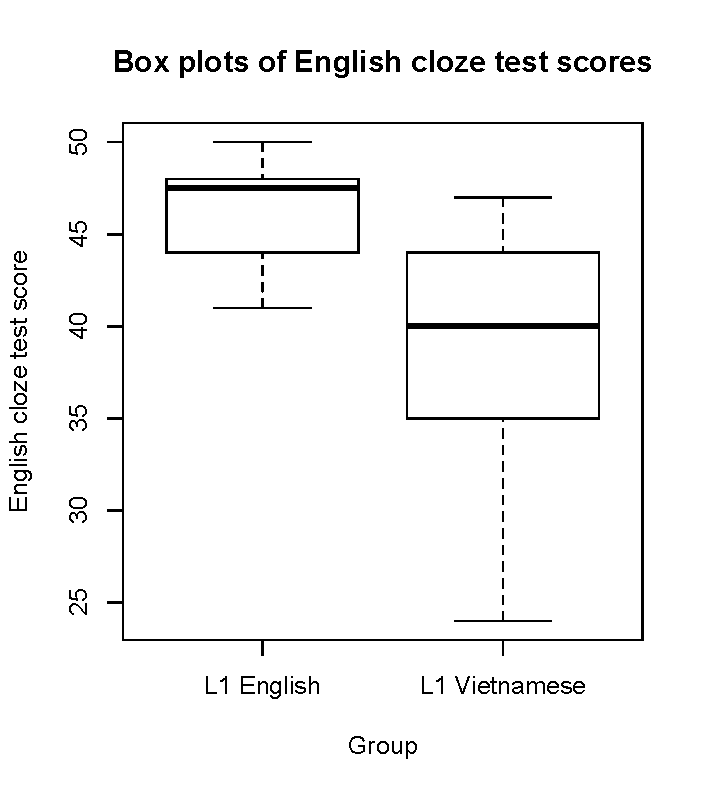
\includegraphics[scale=0.7]{clozetestboxplot.pdf} 
\caption{Box plot of two groups' performance on the English cloze test}
\label{fig:clozeboxplot}
\end{center}   
\end{figure}


\lstinputlisting[frame=tb,frame=tb,caption=Two-tailed t-test result comparing two groups' cloze score means,label=zebra]{cloze-t-test.txt}

Regarding the main test, both groups' performance in the perception task (including the fillers) and stress perception task (only test stimuli are considered) is shown in the box plots \ref{fig:perceptionboxplot} and \ref{fig:stressboxplot}. Again, the L1 English group's score distribution suggests that the L1 English speakers outperformed the L1 Vietnamese group, and the mean score differences were found to be statistically significant (p \textless .05).

\begin{figure}[H]
\begin{center}  
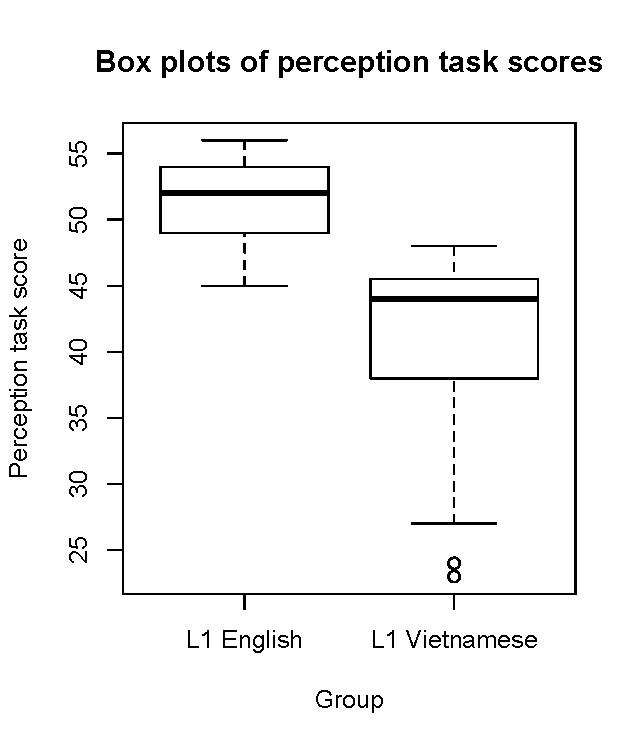
\includegraphics[scale=0.7]{perceptionboxplot.pdf} 
\caption{Box plot of two groups' performance on the main test}
\label{fig:perceptionboxplot}
\end{center}   
\end{figure}

\lstinputlisting[frame=tb,frame=tb,caption=Two-tailed t-test result comparing two groups' perception score means,label=zebra]{perceptionttest.txt}

\begin{figure}[H]
\begin{center}  
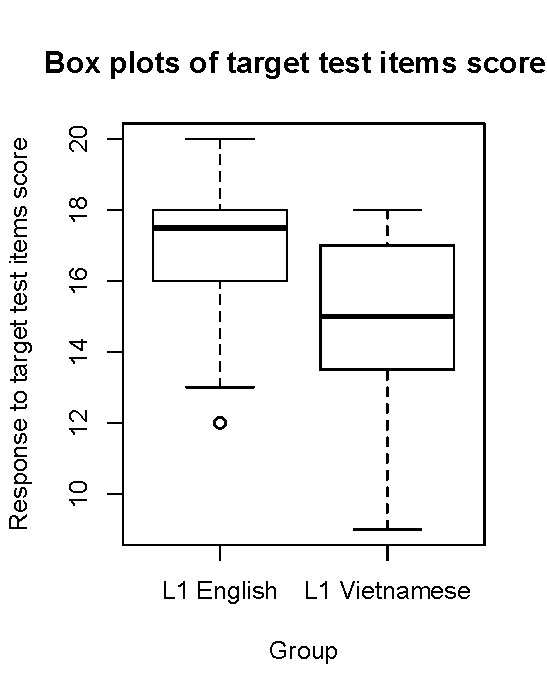
\includegraphics[scale=0.7]{stressboxplot.pdf} 
\caption{Box plot of two groups' performance on the stress perception test}
\label{fig:stressboxplot}
\end{center}   
\end{figure}
 
\lstinputlisting[frame=tb,frame=tb,caption=Two-tailed t-test result comparing two groups' stress perception score means,label=zebra]{stressttest.txt}

\subsubsection{Identification accuracy}

The identification accuracy for bisyllabic words was calculated as the percentage of correct response with respect to matching the word to the same stress pattern, out of the total number of stimuli. For each intonation type, this identification accuracy was calculated out of eight stimuli for bisyllabic words. The figures in \ref{fig:ics} and \ref{fig:icq} show that accuracy was generally lowered for the question intonation, and especially so for the L1 Vietnamese group. The same chart for the trisyllabic words was created and this pattern is quite evident here as well. The identification accuracy for trisyllabic words of each intonation type was calculated out of three stimuli that were presented to each participant. From \ref{fig:icq3}, it can be seen that more than half the participants in the L1 Vietnamese group fails to correctly match trisyllabic words with the correct stress pattern (n = 12 with the identification accuracy being 0), while there was only one such instance in the L1 English group. Most of the L1 English speakers did moderately well, getting two out of three correct for the majority, but this group of stimuli was a challenge for the L1 English speakers too, for very few managed to score 100 percent. The identification accuracy of trisyllabic words in statement intonation among the L1 English speakers looks much better, with more than half of the participants scoring at least two out of three correct.

\begin{figure}[H]
\begin{center}  
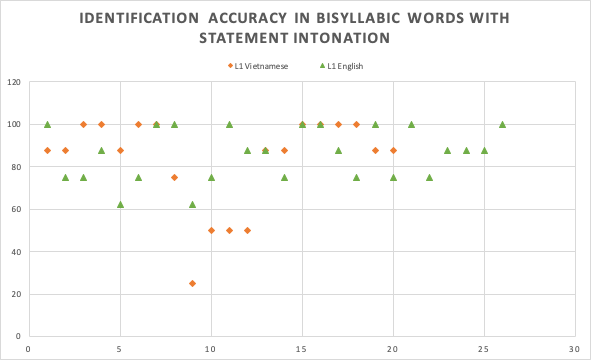
\includegraphics[scale=0.7]{identification-accuracy-statement.png} 
\caption{The identification accuracy for bisyllabic words in statement intonation for both groups}
\label{fig:ics}
\end{center}   
\end{figure}

\begin{figure}[H]
\begin{center}  
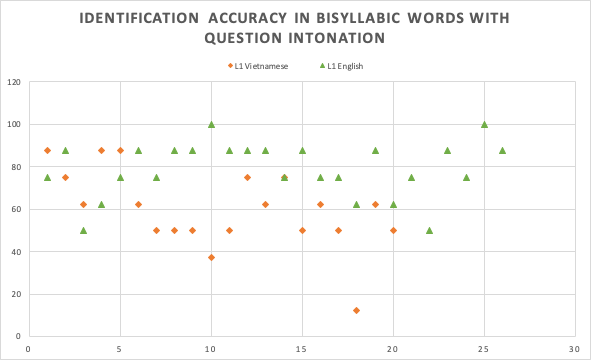
\includegraphics[scale=0.7]{identification-accuracy-question.png} 
\caption{The identification accuracy for bisyllabic words in question intonation for both groups}
\label{fig:icq}
\end{center}   
\end{figure}

\begin{figure}[H]
\begin{center}  
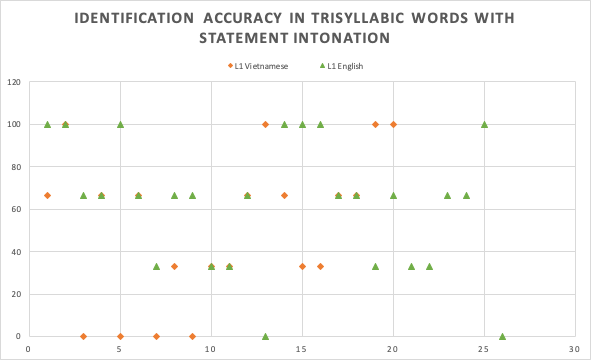
\includegraphics[scale=0.7]{identification-accuracy-tri-statement.png} 
\caption{The identification accuracy for trisyllabic words in statement intonation for both groups}
\label{fig:ics3}
\end{center}   
\end{figure}


\begin{figure}[H]
\begin{center}  
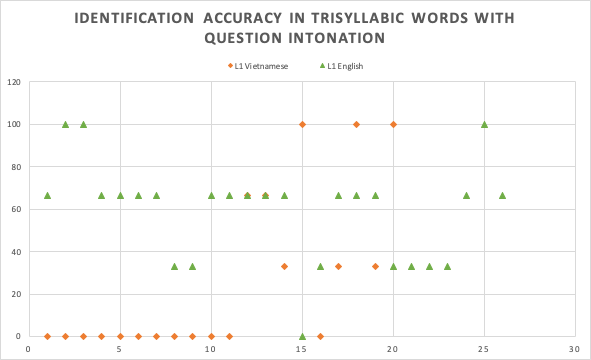
\includegraphics[scale=0.7]{identification-accuracy-tri-question.png} 
\caption{The identification accuracy for trisyllabic words in question intonation for both groups}
\label{fig:icq3}
\end{center}   
\end{figure}

\subsubsection{Mixed effects analysis}

\paragraph{Bisyllabic stimuli} \

In order to answer research question 1, this study examines the performance of participants, by measuring the number of correct responses as dependent variable when varying one between-subjects factor (L1) and two within-subjects factors (the intonation contour type with two levels: sentence or question intonation and the stress location in the word with two levels: initial or final for the bisyllabic words). A general linear mixed ANOVA was run with the aforementioned factors and the results presented below. The sentence intonation level is labeled as SENTENCE, the question intonation level is labeled as QUESTION, the word-initial stress location is labeled as 10, the word-final stress location is labeled as 01, L1 English group is coded as 0, and L1 Vietnamese group is coded as 1 in the subsequent statistical summaries.

In Table \ref{tab:anova-sum-2}, it can be seen that the experiment group's mean scores are lower than the control group's mean scores across conditions, except for the word-final stress, statement intonation condition, where the mean scores of the two groups are about the same.

\begin{table}[H]
  \begin{center}
      \caption{Descriptive statistics of stress perception scores in bisyllabic target stimuli}
        \label{tab:anova-sum-2}
\begin{tabular}{|l|l|r|r|r|} 
\hline
\multicolumn{5}{|c|}{Descriptive Statistics}                                                                                      \\ 
\hline
L1                            & ~     & \multicolumn{1}{c|}{Mean} & \multicolumn{1}{c|}{Std. Deviation} & \multicolumn{1}{c|}{N}  \\ 
\hline
\multirow{3}{*}{STATEMENT.10} & 0     & 3.35                      & 0.629                               & 26                      \\ 
\cline{2-5}
                              & 1     & 3.10                      & 1.294                               & 20                      \\ 
\cline{2-5}
                              & Total & 3.24                      & 0.970                               & 46                      \\ 
\hline
\multirow{3}{*}{STATEMENT.01} & 0     & 3.54                      & 0.706                               & 26                      \\ 
\cline{2-5}
                              & 1     & 3.55                      & 0.759                               & 20                      \\ 
\cline{2-5}
                              & Total & 3.54                      & 0.721                               & 46                      \\ 
\hline
\multirow{3}{*}{QUESTION.10}  & 0     & 3.27                      & 0.827                               & 26                      \\ 
\cline{2-5}
                              & 1     & 2.00                      & 1.124                               & 20                      \\ 
\cline{2-5}
                              & Total & 2.72                      & 1.148                               & 46                      \\ 
\hline
\multirow{3}{*}{QUESTION.01}  & 0     & 3.04                      & 0.774                               & 26                      \\ 
\cline{2-5}
                              & 1     & 2.80                      & 1.005                               & 20                      \\ 
\cline{2-5}
                              & Total & 2.93                      & 0.879                               & 46                      \\
\hline
\end{tabular}
\end{center}
\end{table}

The within-subject effects summary in Table \ref{tab:withinsub2} shows that there is a significant main effect of intonation type, F(1, 44) = 22.7, p \textless .05 on the stress perception score. There is also a statistically significant main effect of the stress position, F(1, 44) = 5.762, p \textless .05. There is no evidence showing any interaction between the within subjects variables, sentence type and stress location, which is also supported by the interaction plot in \ref{fig:interaction2}. On the other hand, there is an interaction effect between the intonation type and the L1 factor, F(1, 44) = 6.254, p \textless .05 and similarly there is an interaction effect between the stress location and the L1 factor as well,  F(1, 44) = 6.517, p \textless .05.


\begin{table}[H]
  \begin{center}
      \caption{Within-subjects effects}
      \label{tab:withinsub2}
\begin{tabular}{p{0.2\textwidth}p{0.2\textwidth}|l|r|r|r|r|r|} 
\hline
\multicolumn{7}{|c|}{Tests of Within-Subjects Effects}                                                                                                                                                                              \\ 
\hline
Measure:~                                               & MEASURE\_1         & \multicolumn{1}{l|}{}             & \multicolumn{1}{l|}{}   & \multicolumn{1}{l|}{}            & \multicolumn{1}{l|}{}  & \multicolumn{1}{l|}{}      \\ 
\hline
Source                                                  & ~                  & \multicolumn{1}{c|}{Type III SoS} & \multicolumn{1}{c|}{df} & \multicolumn{1}{c|}{Mean Square} & \multicolumn{1}{c|}{F} & \multicolumn{1}{c|}{Sig.}  \\ 
\hline
\multirow{4}{*}{Sentence\_type}                         & Sphericity Assumed & 16.646                            & 1                       & 16.646                           & 22.728                 & 0.000                      \\ 
\cline{2-7}
                                                        & Greenhouse-Geisser & 16.646                            & 1.000                   & 16.646                           & 22.728                 & 0.000                      \\ 
\cline{2-7}
                                                        & Huynh-Feldt        & 16.646                            & 1.000                   & 16.646                           & 22.728                 & 0.000                      \\ 
\cline{2-7}
                                                        & Lower-bound        & 16.646                            & 1.000                   & 16.646                           & 22.728                 & 0.000                      \\ 
\hline
\multirow{4}{*}{Sentence\_type * L1}                    & Sphericity Assumed & 4.580                             & 1                       & 4.580                            & 6.254                  & 0.016                      \\ 
\cline{2-7}
                                                        & Greenhouse-Geisser & 4.580                             & 1.000                   & 4.580                            & 6.254                  & 0.016                      \\ 
\cline{2-7}
                                                        & Huynh-Feldt        & 4.580                             & 1.000                   & 4.580                            & 6.254                  & 0.016                      \\ 
\cline{2-7}
                                                        & Lower-bound        & 4.580                             & 1.000                   & 4.580                            & 6.254                  & 0.016                      \\ 
\hline
\multirow{4}{*}{Error(Sentence\_type)}                  & Sphericity Assumed & 32.224                            & 44                      & 0.732                            & \multicolumn{1}{l|}{~} & \multicolumn{1}{l|}{~}     \\ 
\cline{2-7}
                                                        & Greenhouse-Geisser & 32.224                            & 44.000                  & 0.732                            & \multicolumn{1}{l|}{~} & \multicolumn{1}{l|}{~}     \\ 
\cline{2-7}
                                                        & Huynh-Feldt        & 32.224                            & 44.000                  & 0.732                            & \multicolumn{1}{l|}{~} & \multicolumn{1}{l|}{~}     \\ 
\cline{2-7}
                                                        & Lower-bound        & 32.224                            & 44.000                  & 0.732                            & \multicolumn{1}{l|}{~} & \multicolumn{1}{l|}{~}     \\ 
\hline
\multirow{4}{*}{Stress\_location}                       & Sphericity Assumed & 4.148                             & 1                       & 4.148                            & 5.762                  & 0.021                      \\ 
\cline{2-7}
                                                        & Greenhouse-Geisser & 4.148                             & 1.000                   & 4.148                            & 5.762                  & 0.021                      \\ 
\cline{2-7}
                                                        & Huynh-Feldt        & 4.148                             & 1.000                   & 4.148                            & 5.762                  & 0.021                      \\ 
\cline{2-7}
                                                        & Lower-bound        & 4.148                             & 1.000                   & 4.148                            & 5.762                  & 0.021                      \\ 
\hline
\multirow{4}{*}{Stress\_location * L1}                  & Sphericity Assumed & 4.692                             & 1                       & 4.692                            & 6.517                  & 0.014                      \\ 
\cline{2-7}
                                                        & Greenhouse-Geisser & 4.692                             & 1.000                   & 4.692                            & 6.517                  & 0.014                      \\ 
\cline{2-7}
                                                        & Huynh-Feldt        & 4.692                             & 1.000                   & 4.692                            & 6.517                  & 0.014                      \\ 
\cline{2-7}
                                                        & Lower-bound        & 4.692                             & 1.000                   & 4.692                            & 6.517                  & 0.014                      \\ 
\hline
\multirow{4}{*}{Error(Stress\_location)}                & Sphericity Assumed & 31.678                            & 44                      & 0.720                            & \multicolumn{1}{l|}{~} & \multicolumn{1}{l|}{~}     \\ 
\cline{2-7}
                                                        & Greenhouse-Geisser & 31.678                            & 44.000                  & 0.720                            & \multicolumn{1}{l|}{~} & \multicolumn{1}{l|}{~}     \\ 
\cline{2-7}
                                                        & Huynh-Feldt        & 31.678                            & 44.000                  & 0.720                            & \multicolumn{1}{l|}{~} & \multicolumn{1}{l|}{~}     \\ 
\cline{2-7}
                                                        & Lower-bound        & 31.678                            & 44.000                  & 0.720                            & \multicolumn{1}{l|}{~} & \multicolumn{1}{l|}{~}     \\ 
\hline
\multirow{4}{*}{Sentence\_type * Stress\_location}      & Sphericity Assumed & 0.015                             & 1                       & 0.015                            & 0.020                  & 0.887                      \\ 
\cline{2-7}
                                                        & Greenhouse-Geisser & 0.015                             & 1.000                   & 0.015                            & 0.020                  & 0.887                      \\ 
\cline{2-7}
                                                        & Huynh-Feldt        & 0.015                             & 1.000                   & 0.015                            & 0.020                  & 0.887                      \\ 
\cline{2-7}
                                                        & Lower-bound        & 0.015                             & 1.000                   & 0.015                            & 0.020                  & 0.887                      \\ 
\hline
\multirow{4}{*}{Sentence\_type * Stress\_location * L1} & Sphericity Assumed & 1.689                             & 1                       & 1.689                            & 2.271                  & 0.139                      \\ 
\cline{2-7}
                                                        & Greenhouse-Geisser & 1.689                             & 1.000                   & 1.689                            & 2.271                  & 0.139                      \\ 
\cline{2-7}
                                                        & Huynh-Feldt        & 1.689                             & 1.000                   & 1.689                            & 2.271                  & 0.139                      \\ 
\cline{2-7}
                                                        & Lower-bound        & 1.689                             & 1.000                   & 1.689                            & 2.271                  & 0.139                      \\ 
\hline
\multirow{4}{*}{Error(Sentence\_type*Stress\_location)} & Sphericity Assumed & 32.724                            & 44                      & 0.744                            & \multicolumn{1}{l|}{~} & \multicolumn{1}{l|}{~}     \\ 
\cline{2-7}
                                                        & Greenhouse-Geisser & 32.724                            & 44.000                  & 0.744                            & \multicolumn{1}{l|}{~} & \multicolumn{1}{l|}{~}     \\ 
\cline{2-7}
                                                        & Huynh-Feldt        & 32.724                            & 44.000                  & 0.744                            & \multicolumn{1}{l|}{~} & \multicolumn{1}{l|}{~}     \\ 
\cline{2-7}
                                                        & Lower-bound        & 32.724                            & 44.000                  & 0.744                            & \multicolumn{1}{l|}{~} & \multicolumn{1}{l|}{~}     \\
\hline
\end{tabular}
\end{center}
\end{table}


\begin{figure}[H]
\begin{center} 
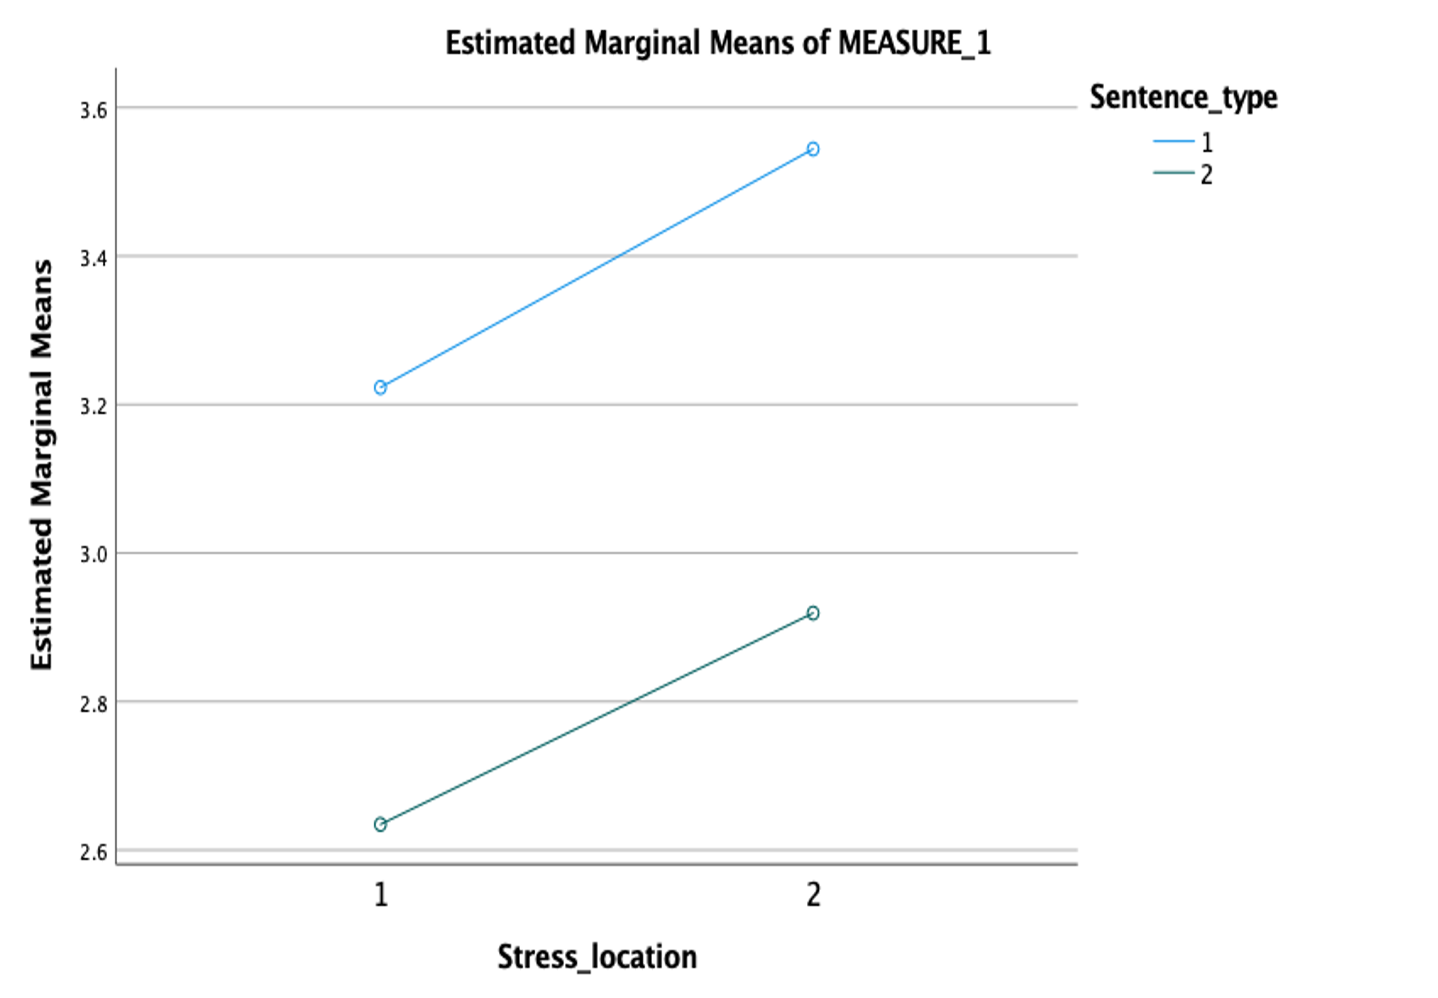
\includegraphics[scale=0.7]{interactionplot.png} 
\caption{Interaction plot}
\label{fig:interaction2}
\end{center}   
\end{figure}


The between-subjects effects summary below shows that there is a statistically significant difference between the stress perception score across the two groups, F(1, 44) =  8.629, p \textless .05, and going by the descriptive statistics, this means there is evidence supporting that the L1 English speakers' stress perception performance is better than the L1 Vietnamese speakers' performance, for bisyllabic words.

\begin{table}[H]
\begin{center}
    \caption{Between-subjects effects}
\begin{tabular}{|l|r|r|r|l|l|} 
\hline
\multicolumn{6}{|c|}{Tests of Between-Subjects Effects}                                                                                                                                          \\ 
\hline
Measure:~              & \multicolumn{1}{l|}{MEASURE\_1}              & \multicolumn{1}{l|}{}   & \multicolumn{1}{l|}{}            &                               &                             \\ 
\hline
Transformed Variable:~ & \multicolumn{1}{l|}{Average}                 & \multicolumn{1}{l|}{}   & \multicolumn{1}{l|}{}            &                               &                             \\ 
\hline
Source                 & \multicolumn{1}{c|}{Type III Sum of Squares} & \multicolumn{1}{c|}{df} & \multicolumn{1}{c|}{Mean Square} & \multicolumn{1}{c|}{F}        & \multicolumn{1}{c|}{Sig.}   \\ 
\hline
Intercept              & 1716.122                                     & 1                       & 1716.122                         & \multicolumn{1}{r|}{1726.043} & \multicolumn{1}{r|}{0.000}  \\ 
\hline
L1                     & 8.579                                        & 1                       & 8.579                            & \multicolumn{1}{r|}{8.629}    & \multicolumn{1}{r|}{0.005}  \\ 
\hline
Error                  & 43.747                                       & 44                      & 0.994                            & ~                             & ~                           \\
\hline
\end{tabular}
\end{center}
\end{table}

To examine the interaction between the L1 factor and intonation type/stress pattern factors, independent samples t-tests with a Bonferroni correction were run. The result summaries below reveal that the source of the interaction is in the question intonation and the word-initial stress location, crossing with the L1 factor. Therefore, there is evidence supporting that L2 speakers performed worse in question intonation and word-intial stress conditions, fully in line with the hypothesis set forth at the beginning of the paper. Detailed results of these independent samples t-tests are presented below.


% question intonation t-test
% descriptive stat

According to the descriptive summary of stress perception scores in Table \ref{tab:stats-intonation-t}, the L1 English speakers scored on average 3 points higher than the L2 English speakers when presented with statement stimuli, and they scored 18 points on average more than the L2 English speakers when presented with \textit{question} stimuli. The t-test, shown in Table \ref{tab:t-condition} shows statistically significant difference in the question intonation category after a Bonferroni correction (t(44) = -4.056, p \textless 0.0125 or 0.05/4), but not in the statement category. The effect size of this difference is quite large, at 17.1892, shown in Table \ref{tab:effect}.

\begin{table}[H]
\centering
\caption{Stress perception scores of L1 English (=0) and L1 Vietnamese (=1) groups for words with different intonation types}
\label{tab:stats-intonation-t}
\begin{tabular}{|l|l|r|r|r|r|} 
\hline
\multicolumn{6}{|c|}{Group Statistics}                                                                                                                                   \\ 
\hline
L1                                &   & \multicolumn{1}{c|}{N} & \multicolumn{1}{c|}{Mean} & \multicolumn{1}{c|}{Std. Deviation} & \multicolumn{1}{c|}{Std. Error Mean}  \\ 
\hline
\multirow{2}{*}{FACTOR.STATEMENT} & 1 & 20                     & 83.125                    & 21.9430                             & 4.9066                                \\ 
\cline{2-6}
                                  & 0 & 26                     & 86.058                    & 12.4132                             & 2.4344                                \\ 
\hline
\multirow{2}{*}{FACTOR.QUESTION}  & 1 & 20                     & 60.000                    & 18.4069                             & 4.1159                                \\ 
\cline{2-6}
                                  & 0 & 26                     & 78.846                    & 13.1193                             & 2.5729                                \\
\hline
\end{tabular}
\end{table}

\begin{table}[H]
\centering
\caption{Independent samples tests result}
\label{tab:stats-intonation-t}
\begin{tabular}{|l|c|c|r|r|r|} 
\hline
\multicolumn{6}{|c|}{Independent Samples Test}                                                                                                                                                                                                 \\ 
\hline
                                  & \multicolumn{2}{c|}{Levene's Test for Equality of Variances} & \multicolumn{3}{c|}{t-test for Equality of Means}                                                                                           \\ 
\hline
                                  & \multirow{2}{*}{F}         & \multirow{2}{*}{Sig.}           & \multicolumn{1}{c|}{\multirow{2}{*}{t}} & \multicolumn{1}{c|}{\multirow{2}{*}{df}} & \multicolumn{1}{c|}{\multirow{2}{*}{Sig. (2-tailed)}}  \\ 
\cline{1-1}
                                  &                            &                                 & \multicolumn{1}{c|}{}                   & \multicolumn{1}{c|}{}                    & \multicolumn{1}{c|}{}                                  \\ 
\hline
\multirow{2}{*}{FACTOR.STATEMENT} & \multicolumn{1}{r|}{3.993} & \multicolumn{1}{r|}{0.052}      & -0.574                                  & 44                                       & 0.569                                                  \\ 
\cline{2-6}
                                  & \multicolumn{1}{l|}{~}     & \multicolumn{1}{l|}{~}          & -0.535                                  & 28.207                                   & 0.597                                                  \\ 
\hline
\multirow{2}{*}{FACTOR.QUESTION}  & \multicolumn{1}{r|}{1.490} & \multicolumn{1}{r|}{0.229}      & -4.056                                  & 44                                       & 0.000                                                  \\ 
\cline{2-6}
                                  & \multicolumn{1}{l|}{~}     & \multicolumn{1}{l|}{~}          & -3.883                                  & 32.929                                   & 0.000                                                  \\
\hline
\end{tabular}
\end{table}

% effect size
\begin{table}[H]
\centering
\caption{Independent samples effect sizes}
\label{tab:effect}
\begin{tabular}{|l|l|r|r|r|r|} 
\hline
\multicolumn{6}{|c|}{Independent Samples Effect Sizes}                                                                                                                                                                         \\ 
\hline
                                  &                    & \multicolumn{1}{c|}{\multirow{2}{*}{Standardizera}} & \multicolumn{1}{c|}{\multirow{2}{*}{Point Estimate}} & \multicolumn{2}{c|}{95\% Confidence Interval}            \\ 
\cline{1-2}\cline{5-6}
                                  &                    & \multicolumn{1}{c|}{}                               & \multicolumn{1}{c|}{}                                & \multicolumn{1}{c|}{Lower} & \multicolumn{1}{c|}{Upper}  \\ 
\hline
\multirow{3}{*}{FACTOR.STATEMENT} & Cohen's d          & 17.1892                                             & -0.171                                               & -0.754                     & 0.414                       \\ 
\cline{2-6}
                                  & Hedges' correction & 17.4893                                             & -0.168                                               & -0.741                     & 0.407                       \\ 
\cline{2-6}
                                  & Glass's delta      & 12.4132                                             & -0.236                                               & -0.821                     & 0.353                       \\ 
\hline
\multirow{3}{*}{FACTOR.QUESTION}  & Cohen's d          & 15.6237                                             & -1.206                                               & -1.835                     & -0.566                      \\ 
\cline{2-6}
                                  & Hedges' correction & 15.8965                                             & -1.186                                               & -1.804                     & -0.556                      \\ 
\cline{2-6}
                                  & Glass's delta      & 13.1193                                             & -1.437                                               & -2.131                     & -0.722                      \\
\hline
\end{tabular}
\end{table}


According to the descriptive summary of stress perception scores by stress location in Table \ref{tab:location}, the L1 English speakers scored on average about 21 points higher than the L2 English speakers when presented with word-intial stress stimuli, and they scored 3 points on average more than the L2 English speakers when presented with word-final stress stimuli. The t-test, shown in Table \ref{tab:location} shows statistically significant difference in the word-intial category after a Bonferroni correction (t(44) = -4.056, p \textless 0.0125), but not in the word-final category. The effect size of this difference is quite large, at 16.8501, shown in Table \ref{tab:effect-location}.

%descriptive stat stress location
\begin{table}[H]
\centering
\caption{Stress perception scores of L1 English (=0) and L1 Vietnamese (=1) groups for words with different stress locations}
\label{tab:location}
\begin{tabular}{|l|l|r|r|r|r|} 
\hline
\multicolumn{6}{|c|}{Group Statistics}                                                                                                                            \\ 
\hline
L1                         &   & \multicolumn{1}{c|}{N} & \multicolumn{1}{c|}{Mean} & \multicolumn{1}{c|}{Std. Deviation} & \multicolumn{1}{c|}{Std. Error Mean}  \\ 
\hline
\multirow{2}{*}{FACTOR.10} & 1 & 20                     & 63.750                    & 21.0341                             & 4.7034                                \\ 
\cline{2-6}
                           & 0 & 26                     & 82.692                    & 12.7852                             & 2.5074                                \\ 
\hline
\multirow{2}{*}{FACTOR.01} & 1 & 20                     & 79.375                    & 16.8561                             & 3.7691                                \\ 
\cline{2-6}
                           & 0 & 26                     & 82.212                    & 15.0719                             & 2.9559                                \\
\hline
\end{tabular}

\end{table}

% t test stress location
\begin{table}[H]
\centering
\caption{Independent samples tests result}
\label{tab:location}
\begin{tabular}{|l|c|c|r|r|r|} 
\hline
\multicolumn{6}{|c|}{Independent Samples Test}                                                                                                                                                                                          \\ 
\hline
                           & \multicolumn{2}{c|}{Levene's Test for Equality of Variances} & \multicolumn{3}{c|}{t-test for Equality of Means}                                                                                           \\ 
\hline
                           & \multirow{2}{*}{F}         & \multirow{2}{*}{Sig.}           & \multicolumn{1}{c|}{\multirow{2}{*}{t}} & \multicolumn{1}{c|}{\multirow{2}{*}{df}} & \multicolumn{1}{c|}{\multirow{2}{*}{Sig. (2-tailed)}}  \\ 
\cline{1-1}
                           &                            &                                 & \multicolumn{1}{c|}{}                   & \multicolumn{1}{c|}{}                    & \multicolumn{1}{c|}{}                                  \\ 
\hline
\multirow{2}{*}{FACTOR.10} & \multicolumn{1}{r|}{7.733} & \multicolumn{1}{r|}{0.008}      & -3.780                                  & 44                                       & 0.000                                                  \\ 
\cline{2-6}
                           & \multicolumn{1}{l|}{~}     & \multicolumn{1}{l|}{~}          & -3.554                                  & 29.522                                   & 0.001                                                  \\ 
\hline
\multirow{2}{*}{FACTOR.01} & \multicolumn{1}{r|}{0.418} & \multicolumn{1}{r|}{0.521}      & -0.601                                  & 44                                       & 0.551                                                  \\ 
\cline{2-6}
                           & \multicolumn{1}{l|}{~}     & \multicolumn{1}{l|}{~}          & -0.592                                  & 38.492                                   & 0.557                                                  \\
\hline
\end{tabular}
\end{table}

% effect size
\begin{table}[H]
\centering
\caption{Independent samples effect sizes}
\label{tab:effect-location}
\begin{tabular}{|l|l|r|r|r|r|} 
\hline
\multicolumn{6}{|c|}{Independent Samples Effect Sizes}                                                                                                                                                                  \\ 
\hline
                           &                    & \multicolumn{1}{c|}{\multirow{2}{*}{Standardizera}} & \multicolumn{1}{c|}{\multirow{2}{*}{Point Estimate}} & \multicolumn{2}{c|}{95\% Confidence Interval}            \\ 
\cline{1-2}\cline{5-6}
                           &                    & \multicolumn{1}{c|}{}                               & \multicolumn{1}{c|}{}                                & \multicolumn{1}{c|}{Lower} & \multicolumn{1}{c|}{Upper}  \\ 
\hline
\multirow{3}{*}{FACTOR.10} & Cohen's d          & 16.8501                                             & -1.124                                               & -1.747                     & -0.490                      \\ 
\cline{2-6}
                           & Hedges' correction & 17.1443                                             & -1.105                                               & -1.717                     & -0.482                      \\ 
\cline{2-6}
                           & Glass's delta      & 12.7852                                             & -1.482                                               & -2.183                     & -0.760                      \\ 
\hline
\multirow{3}{*}{FACTOR.01} & Cohen's d          & 15.8670                                             & -0.179                                               & -0.762                     & 0.406                       \\ 
\cline{2-6}
                           & Hedges' correction & 16.1440                                             & -0.176                                               & -0.749                     & 0.399                       \\ 
\cline{2-6}
                           & Glass's delta      & 15.0719                                             & -0.188                                               & -0.772                     & 0.399                       \\
\hline
\end{tabular}
\end{table}

The mixed effects ANOVA analysis on bisyllabic words suggests that there is a clear difference in stress perception performance between the two groups of participants, where the L1 English speakers performed better than the L1 Vietnamese speakers. Notably, the analysis gives support to the hypothesis that the difference between the two groups are due to the question intonation condition and the word-initial condition. The effect size of this result is large, suggesting that it is quite robust. 
% Save this for the discussion: We have evidence that the word-initial and question intonation condition can explain the difference in performance between the  

%% THREE SYLLABLE ANALYSIS
\paragraph{Trisyllabic stimuli} \

A mixed effects ANOVA analysis was performed on the trisyllabic stimuli, but no significant differences were found among the within subjects variables (see Table \ref{tab:within3}). Performance based on the mean scores between the two groups looks quite comparable, as seen in Table \ref{tab:tri-descriptive} and the between subject variable (L1) also doesn't show any significant effect (see Table \ref{tab:between3}).

% mention the reason in the discussion. 

\begin{table}[H]
\begin{center}
      \caption{Descriptive statistics of perception scores in trisyllabic target stimuli}
      \label{tab:tri-descriptive}
\begin{tabular}{|l|l|r|r|r|} 
\hline
\multicolumn{5}{|c|}{Descriptive Statistics}                                                                                       \\ 
\hline
L1                             &       & \multicolumn{1}{c|}{Mean} & \multicolumn{1}{c|}{Std. Deviation} & \multicolumn{1}{c|}{N}  \\ 
\hline
\multirow{3}{*}{STATEMENT.100} & 0     & 0.65                      & 0.485                               & 26                      \\ 
\cline{2-5}
                               & 1     & 0.40                      & 0.503                               & 20                      \\ 
\cline{2-5}
                               & Total & 0.54                      & 0.504                               & 46                      \\ 
\hline
\multirow{3}{*}{STATEMENT.010} & 0     & 0.77                      & 0.430                               & 26                      \\ 
\cline{2-5}
                               & 1     & 0.45                      & 0.510                               & 20                      \\ 
\cline{2-5}
                               & Total & 0.63                      & 0.488                               & 46                      \\ 
\hline
\multirow{3}{*}{STATEMENT.001} & 0     & 0.58                      & 0.504                               & 26                      \\ 
\cline{2-5}
                               & 1     & 0.65                      & 0.489                               & 20                      \\ 
\cline{2-5}
                               & Total & 0.61                      & 0.493                               & 46                      \\ 
\hline
\multirow{3}{*}{QUESTION.100}  & 0     & 0.50                      & 0.510                               & 26                      \\ 
\cline{2-5}
                               & 1     & 0.45                      & 0.510                               & 20                      \\ 
\cline{2-5}
                               & Total & 0.48                      & 0.505                               & 46                      \\ 
\hline
\multirow{3}{*}{QUESTION.010}  & 0     & 0.58                      & 0.504                               & 26                      \\ 
\cline{2-5}
                               & 1     & 0.40                      & 0.503                               & 20                      \\ 
\cline{2-5}
                               & Total & 0.50                      & 0.506                               & 46                      \\ 
\hline
\multirow{3}{*}{QUESTION.001}  & 0     & 0.69                      & 0.471                               & 26                      \\ 
\cline{2-5}
                               & 1     & 0.65                      & 0.489                               & 20                      \\ 
\cline{2-5}
                               & Total & 0.67                      & 0.474                               & 46                      \\
\hline
\end{tabular}
\end{center}
\end{table}

%% withint subjects for 3 syllable


\begin{table}[H]
\centering
\caption{Within-subjects effects}
\label{tab:within3}
\begin{tabular}{p{0.2\textwidth}p{0.2\textwidth}|l|r|r|r|r|r|} 
\hline
\multicolumn{7}{|c|}{Tests of Within-Subjects Effects}                                                                                                                                                                                         \\ 
\hline
Measure:~                                               & MEASURE\_1         & \multicolumn{1}{l|}{}                        & \multicolumn{1}{l|}{}   & \multicolumn{1}{l|}{}            & \multicolumn{1}{l|}{}  & \multicolumn{1}{l|}{}      \\ 
\hline
Source                                                  & ~                  & \multicolumn{1}{c|}{Type III SoS} & \multicolumn{1}{c|}{df} & \multicolumn{1}{c|}{Mean Square} & \multicolumn{1}{c|}{F} & \multicolumn{1}{c|}{Sig.}  \\ 
\hline
\multirow{4}{*}{Sentence\_type}                         & Sphericity Assumed & 0.100                                        & 1                       & 0.100                            & 0.568                  & 0.455                      \\ 
\cline{2-7}
                                                        & Greenhouse-Geisser & 0.100                                        & 1.000                   & 0.100                            & 0.568                  & 0.455                      \\ 
\cline{2-7}
                                                        & Huynh-Feldt        & 0.100                                        & 1.000                   & 0.100                            & 0.568                  & 0.455                      \\ 
\cline{2-7}
                                                        & Lower-bound        & 0.100                                        & 1.000                   & 0.100                            & 0.568                  & 0.455                      \\ 
\hline
\multirow{4}{*}{Sentence\_type * L1}                    & Sphericity Assumed & 0.100                                        & 1                       & 0.100                            & 0.568                  & 0.455                      \\ 
\cline{2-7}
                                                        & Greenhouse-Geisser & 0.100                                        & 1.000                   & 0.100                            & 0.568                  & 0.455                      \\ 
\cline{2-7}
                                                        & Huynh-Feldt        & 0.100                                        & 1.000                   & 0.100                            & 0.568                  & 0.455                      \\ 
\cline{2-7}
                                                        & Lower-bound        & 0.100                                        & 1.000                   & 0.100                            & 0.568                  & 0.455                      \\ 
\hline
\multirow{4}{*}{Error(Sentence\_type)}                  & Sphericity Assumed & 7.769                                        & 44                      & 0.177                            & \multicolumn{1}{l|}{~} & \multicolumn{1}{l|}{~}     \\ 
\cline{2-7}
                                                        & Greenhouse-Geisser & 7.769                                        & 44.000                  & 0.177                            & \multicolumn{1}{l|}{~} & \multicolumn{1}{l|}{~}     \\ 
\cline{2-7}
                                                        & Huynh-Feldt        & 7.769                                        & 44.000                  & 0.177                            & \multicolumn{1}{l|}{~} & \multicolumn{1}{l|}{~}     \\ 
\cline{2-7}
                                                        & Lower-bound        & 7.769                                        & 44.000                  & 0.177                            & \multicolumn{1}{l|}{~} & \multicolumn{1}{l|}{~}     \\ 
\hline
\multirow{4}{*}{Stress\_location}                       & Sphericity Assumed & 0.934                                        & 2                       & 0.467                            & 2.557                  & 0.083                      \\ 
\cline{2-7}
                                                        & Greenhouse-Geisser & 0.934                                        & 1.889                   & 0.494                            & 2.557                  & 0.087                      \\ 
\cline{2-7}
                                                        & Huynh-Feldt        & 0.934                                        & 2.000                   & 0.467                            & 2.557                  & 0.083                      \\ 
\cline{2-7}
                                                        & Lower-bound        & 0.934                                        & 1.000                   & 0.934                            & 2.557                  & 0.117                      \\ 
\hline
\multirow{4}{*}{Stress\_location * L1}                  & Sphericity Assumed & 0.804                                        & 2                       & 0.402                            & 2.200                  & 0.117                      \\ 
\cline{2-7}
                                                        & Greenhouse-Geisser & 0.804                                        & 1.889                   & 0.425                            & 2.200                  & 0.120                      \\ 
\cline{2-7}
                                                        & Huynh-Feldt        & 0.804                                        & 2.000                   & 0.402                            & 2.200                  & 0.117                      \\ 
\cline{2-7}
                                                        & Lower-bound        & 0.804                                        & 1.000                   & 0.804                            & 2.200                  & 0.145                      \\ 
\hline
\multirow{4}{*}{Error(Stress\_location)}                & Sphericity Assumed & 16.073                                       & 88                      & 0.183                            & \multicolumn{1}{l|}{~} & \multicolumn{1}{l|}{~}     \\ 
\cline{2-7}
                                                        & Greenhouse-Geisser & 16.073                                       & 83.127                  & 0.193                            & \multicolumn{1}{l|}{~} & \multicolumn{1}{l|}{~}     \\ 
\cline{2-7}
                                                        & Huynh-Feldt        & 16.073                                       & 88.000                  & 0.183                            & \multicolumn{1}{l|}{~} & \multicolumn{1}{l|}{~}     \\ 
\cline{2-7}
                                                        & Lower-bound        & 16.073                                       & 44.000                  & 0.365                            & \multicolumn{1}{l|}{~} & \multicolumn{1}{l|}{~}     \\ 
\hline
\multirow{4}{*}{Sentence\_type * Stress\_location}      & Sphericity Assumed & 0.368                                        & 2                       & 0.184                            & 0.617                  & 0.542                      \\ 
\cline{2-7}
                                                        & Greenhouse-Geisser & 0.368                                        & 1.905                   & 0.193                            & 0.617                  & 0.534                      \\ 
\cline{2-7}
                                                        & Huynh-Feldt        & 0.368                                        & 2.000                   & 0.184                            & 0.617                  & 0.542                      \\ 
\cline{2-7}
                                                        & Lower-bound        & 0.368                                        & 1.000                   & 0.368                            & 0.617                  & 0.436                      \\ 
\hline
\multirow{4}{*}{Sentence\_type * Stress\_location * L1} & Sphericity Assumed & 0.324                                        & 2                       & 0.162                            & 0.544                  & 0.582                      \\ 
\cline{2-7}
                                                        & Greenhouse-Geisser & 0.324                                        & 1.905                   & 0.170                            & 0.544                  & 0.574                      \\ 
\cline{2-7}
                                                        & Huynh-Feldt        & 0.324                                        & 2.000                   & 0.162                            & 0.544                  & 0.582                      \\ 
\cline{2-7}
                                                        & Lower-bound        & 0.324                                        & 1.000                   & 0.324                            & 0.544                  & 0.465                      \\ 
\hline
\multirow{4}{*}{Error(Sentence\_type*Stress\_location)} & Sphericity Assumed & 26.219                                       & 88                      & 0.298                            & \multicolumn{1}{l|}{~} & \multicolumn{1}{l|}{~}     \\ 
\cline{2-7}
                                                        & Greenhouse-Geisser & 26.219                                       & 83.820                  & 0.313                            & \multicolumn{1}{l|}{~} & \multicolumn{1}{l|}{~}     \\ 
\cline{2-7}
                                                        & Huynh-Feldt        & 26.219                                       & 88.000                  & 0.298                            & \multicolumn{1}{l|}{~} & \multicolumn{1}{l|}{~}     \\ 
\cline{2-7}
                                                        & Lower-bound        & 26.219                                       & 44.000                  & 0.596                            & \multicolumn{1}{l|}{~} & \multicolumn{1}{l|}{~}     \\
\hline
\end{tabular}
\end{table}

% between subject three syllable


\begin{table}[H]
\centering
\caption{Between-subjects effects}
\label{tab:between3}
\begin{tabular}{|l|r|r|r|l|l|} 
\hline
\multicolumn{6}{|c|}{Tests of Between-Subjects Effects}                                                                                                                                         \\ 
\hline
Measure:~              & \multicolumn{1}{l|}{MEASURE\_1}              & \multicolumn{1}{l|}{}   & \multicolumn{1}{l|}{}            &                              &                             \\ 
\hline
Transformed Variable:~ & \multicolumn{1}{l|}{Average}                 & \multicolumn{1}{l|}{}   & \multicolumn{1}{l|}{}            &                              &                             \\ 
\hline
Source                 & \multicolumn{1}{c|}{Type III Sum of Squares} & \multicolumn{1}{c|}{df} & \multicolumn{1}{c|}{Mean Square} & \multicolumn{1}{c|}{F}       & \multicolumn{1}{c|}{Sig.}   \\ 
\hline
Intercept              & 86.332                                       & 1                       & 86.332                           & \multicolumn{1}{r|}{275.877} & \multicolumn{1}{r|}{0.000}  \\ 
\hline
L1                     & 1.115                                        & 1                       & 1.115                            & \multicolumn{1}{r|}{3.562}   & \multicolumn{1}{r|}{0.066}  \\ 
\hline
Error                  & 13.769                                       & 44                      & 0.313                            & ~                            & ~                           \\
\hline
\end{tabular}
\end{table}


\paragraph{Reaction time in bisyllabic stimuli} \

In order to answer research question 2, `Would difficulty in identifying the stress location in the yes/no question context manifest in a delayed reaction to the stimuli in the L2 English group?' , various reaction time measures were examined. The participants' reaction time was measured by activating the Question: Timing feature in Qualtrics. According to Qualtrics, this feature gives userrs four metrics:

\begin{enumerate}
\item First Click: Number of seconds from when the page loads to the first click 
\item Last Click: Number of seconds from when the page loads to the click before the “Next” button is selected 
\item Page Submit: Number of seconds from when the page loads to when the “Next” button is selected 
\item Click Count: Number of a respondent clicks on a page 
\end{enumerate}

In this study, three metrics were specifically examined, First Click, Last Click, and Click Count. The first click should give an indication of how fast the participant makes a decision from the moment the audio is played. The click count should gives an indication about how many times the participant changes their mind in the course of answering the question. The last click should give an indication about the total time elapsed since the audio is played, or the total reaction time. The expectation is that L2 English speakers would take longer to answer questions, especially in the QUESTION.10 condition. However, this prediction did not bore out. What seems to be significant is L2 English speakers' likelihood for more a click count more than 1, in other words, they might be more likely to change their minds about the answers, compared to the L1 group. Looking at the descriptive data, the L1 English speakers typically took longer to answer questions than the L2 English speakers, however there was no evidence supporting that this difference was statistically significant. Mixed effects ANOVA models are presented below, as well as followed up post hoc tests, to illustrate the points just made.

%% FIRST CLICK
Table \ref{tab:descriptivefirstclick} shows that L1 English speakers take longer on average than L1 Vietnamese speakers for the first click, except for the QUESTION.10 condition, when both groups take roughly the same time for the first click, on average. Table \ref{tab:betweenfirstclick}, however, does not give support for the difference between the two groups, the p-value is 0.347 \textgreater 0.05 and we cannot reject the null hypothesis that there was no difference in the time to the first click based on L1 factor.

\begin{table}[H]
\centering
\caption{First click in four conditions}
\label{tab:descriptivefirstclick}
\begin{tabular}{|l|l|r|r|r|} 
\hline
\multicolumn{5}{|c|}{Descriptive Statistics}                                                                                                 \\ 
\hline
L1                                       &       & \multicolumn{1}{c|}{Mean} & \multicolumn{1}{c|}{Std. Deviation} & \multicolumn{1}{c|}{N}  \\ 
\hline
\multirow{3}{*}{FIRSTCLICK.STATEMENT.10} & 0     & 11.16150                  & 9.637444                            & 26                      \\ 
\cline{2-5}
                                         & 1     & 8.50850                   & 4.605819                            & 20                      \\ 
\cline{2-5}
                                         & Total & 10.00802                  & 7.894627                            & 46                      \\ 
\hline
\multirow{3}{*}{FIRSTCLICK.STATEMENT.01} & 0     & 10.05042                  & 8.143267                            & 26                      \\ 
\cline{2-5}
                                         & 1     & 9.47900                   & 6.168538                            & 20                      \\ 
\cline{2-5}
                                         & Total & 9.80198                   & 7.279312                            & 46                      \\ 
\hline
\multirow{3}{*}{FIRSTCLICK.QUESTION.10}  & 0     & 15.27388                  & 13.417920                           & 26                      \\ 
\cline{2-5}
                                         & 1     & 14.31685                  & 11.139615                           & 20                      \\ 
\cline{2-5}
                                         & Total & 14.85778                  & 12.355024                           & 46                      \\ 
\hline
\multirow{3}{*}{FIRSTCLICK.QUESTION.01}  & 0     & 13.37965                  & 7.712741                            & 26                      \\ 
\cline{2-5}
                                         & 1     & 9.47255                   & 3.395079                            & 20                      \\ 
\cline{2-5}
                                         & Total & 11.68091                  & 6.461390                            & 46                      \\
\hline
\end{tabular}
\end{table}


Table \ref{tab:withinfirstclick} shows that there are main effects from two within subject variables, the sentence type and stress location factors. For the sentence type, F(1, 44) =  10.677, p \textless .05; and for the stress location factor, F(1, 44) = 5.456, p \textless .05. A followed up pairwise comparison of within subjects factors was conducted and two crossed-conditions were found to be significant.

% First click between variable

\begin{table}[H]
\centering
\caption{Tests of Between-Subjects Effects, Dependent variable: First Click}
\label{tab:betweenfirstclick}
\begin{tabular}{|l|r|r|r|l|l|} 
\hline
\multicolumn{6}{|c|}{Tests of Between-Subjects Effects}                                                                                                                                         \\ 
\hline
Measure:~              & \multicolumn{1}{l|}{MEASURE\_1}              & \multicolumn{1}{l|}{}   & \multicolumn{1}{l|}{}            &                              &                             \\ 
\hline
Transformed Variable:~ & \multicolumn{1}{l|}{Average}                 & \multicolumn{1}{l|}{}   & \multicolumn{1}{l|}{}            &                              &                             \\ 
\hline
Source                 & \multicolumn{1}{c|}{Type III Sum of Squares} & \multicolumn{1}{c|}{df} & \multicolumn{1}{c|}{Mean Square} & \multicolumn{1}{c|}{F}       & \multicolumn{1}{c|}{Sig.}   \\ 
\hline
Intercept              & 23734.389                                    & 1                       & 23734.389                        & \multicolumn{1}{r|}{115.916} & \multicolumn{1}{r|}{0.000}  \\ 
\hline
L1                     & 184.896                                      & 1                       & 184.896                          & \multicolumn{1}{r|}{0.903}   & \multicolumn{1}{r|}{0.347}  \\ 
\hline
Error                  & 9009.187                                     & 44                      & 204.754                          & ~                            & ~                           \\
\hline
\end{tabular}
\end{table}

% firste click within effects

\begin{table}[H]
\centering
\caption{Tests of Within-Subjects Effects, Dependent variable: First Click}
\label{tab:withinfirstclick}
\begin{tabular}{p{0.2\textwidth}p{0.2\textwidth}|l|r|r|r|r|r|} 
\hline
\multicolumn{7}{|c|}{Tests of Within-Subjects Effects}                                                                                                                                                                                         \\ 
\hline
Measure:~                                               & MEASURE\_1         & \multicolumn{1}{l|}{}                        & \multicolumn{1}{l|}{}   & \multicolumn{1}{l|}{}            & \multicolumn{1}{l|}{}  & \multicolumn{1}{l|}{}      \\ 
\hline
Source                                                  & ~                  & \multicolumn{1}{c|}{Type III SoS} & \multicolumn{1}{c|}{df} & \multicolumn{1}{c|}{Mean Square} & \multicolumn{1}{c|}{F} & \multicolumn{1}{c|}{Sig.}  \\ 
\hline
\multirow{4}{*}{Sentence\_type}                         & Sphericity Assumed & 495.669                                      & 1                       & 495.669                          & 10.677                 & 0.002                      \\ 
\cline{2-7}
                                                        & Greenhouse-Geisser & 495.669                                      & 1.000                   & 495.669                          & 10.677                 & 0.002                      \\ 
\cline{2-7}
                                                        & Huynh-Feldt        & 495.669                                      & 1.000                   & 495.669                          & 10.677                 & 0.002                      \\ 
\cline{2-7}
                                                        & Lower-bound        & 495.669                                      & 1.000                   & 495.669                          & 10.677                 & 0.002                      \\ 
\hline
\multirow{4}{*}{Sentence\_type * L1}                    & Sphericity Assumed & 7.598                                        & 1                       & 7.598                            & 0.164                  & 0.688                      \\ 
\cline{2-7}
                                                        & Greenhouse-Geisser & 7.598                                        & 1.000                   & 7.598                            & 0.164                  & 0.688                      \\ 
\cline{2-7}
                                                        & Huynh-Feldt        & 7.598                                        & 1.000                   & 7.598                            & 0.164                  & 0.688                      \\ 
\cline{2-7}
                                                        & Lower-bound        & 7.598                                        & 1.000                   & 7.598                            & 0.164                  & 0.688                      \\ 
\hline
\multirow{4}{*}{Error(Sentence\_type)}                  & Sphericity Assumed & 2042.648                                     & 44                      & 46.424                           & \multicolumn{1}{l|}{~} & \multicolumn{1}{l|}{~}     \\ 
\cline{2-7}
                                                        & Greenhouse-Geisser & 2042.648                                     & 44.000                  & 46.424                           & \multicolumn{1}{l|}{~} & \multicolumn{1}{l|}{~}     \\ 
\cline{2-7}
                                                        & Huynh-Feldt        & 2042.648                                     & 44.000                  & 46.424                           & \multicolumn{1}{l|}{~} & \multicolumn{1}{l|}{~}     \\ 
\cline{2-7}
                                                        & Lower-bound        & 2042.648                                     & 44.000                  & 46.424                           & \multicolumn{1}{l|}{~} & \multicolumn{1}{l|}{~}     \\ 
\hline
\multirow{4}{*}{Stress\_location}                       & Sphericity Assumed & 133.736                                      & 1                       & 133.736                          & 5.456                  & 0.024                      \\ 
\cline{2-7}
                                                        & Greenhouse-Geisser & 133.736                                      & 1.000                   & 133.736                          & 5.456                  & 0.024                      \\ 
\cline{2-7}
                                                        & Huynh-Feldt        & 133.736                                      & 1.000                   & 133.736                          & 5.456                  & 0.024                      \\ 
\cline{2-7}
                                                        & Lower-bound        & 133.736                                      & 1.000                   & 133.736                          & 5.456                  & 0.024                      \\ 
\hline
\multirow{4}{*}{Stress\_location * L1}                  & Sphericity Assumed & 2.132                                        & 1                       & 2.132                            & 0.087                  & 0.769                      \\ 
\cline{2-7}
                                                        & Greenhouse-Geisser & 2.132                                        & 1.000                   & 2.132                            & 0.087                  & 0.769                      \\ 
\cline{2-7}
                                                        & Huynh-Feldt        & 2.132                                        & 1.000                   & 2.132                            & 0.087                  & 0.769                      \\ 
\cline{2-7}
                                                        & Lower-bound        & 2.132                                        & 1.000                   & 2.132                            & 0.087                  & 0.769                      \\ 
\hline
\multirow{4}{*}{Error(Stress\_location)}                & Sphericity Assumed & 1078.572                                     & 44                      & 24.513                           & \multicolumn{1}{l|}{~} & \multicolumn{1}{l|}{~}     \\ 
\cline{2-7}
                                                        & Greenhouse-Geisser & 1078.572                                     & 44.000                  & 24.513                           & \multicolumn{1}{l|}{~} & \multicolumn{1}{l|}{~}     \\ 
\cline{2-7}
                                                        & Huynh-Feldt        & 1078.572                                     & 44.000                  & 24.513                           & \multicolumn{1}{l|}{~} & \multicolumn{1}{l|}{~}     \\ 
\cline{2-7}
                                                        & Lower-bound        & 1078.572                                     & 44.000                  & 24.513                           & \multicolumn{1}{l|}{~} & \multicolumn{1}{l|}{~}     \\ 
\hline
\multirow{4}{*}{Sentence\_type * Stress\_location}      & Sphericity Assumed & 123.028                                      & 1                       & 123.028                          & 3.514                  & 0.067                      \\ 
\cline{2-7}
                                                        & Greenhouse-Geisser & 123.028                                      & 1.000                   & 123.028                          & 3.514                  & 0.067                      \\ 
\cline{2-7}
                                                        & Huynh-Feldt        & 123.028                                      & 1.000                   & 123.028                          & 3.514                  & 0.067                      \\ 
\cline{2-7}
                                                        & Lower-bound        & 123.028                                      & 1.000                   & 123.028                          & 3.514                  & 0.067                      \\ 
\hline
\multirow{4}{*}{Sentence\_type * Stress\_location * L1} & Sphericity Assumed & 71.549                                       & 1                       & 71.549                           & 2.044                  & 0.160                      \\ 
\cline{2-7}
                                                        & Greenhouse-Geisser & 71.549                                       & 1.000                   & 71.549                           & 2.044                  & 0.160                      \\ 
\cline{2-7}
                                                        & Huynh-Feldt        & 71.549                                       & 1.000                   & 71.549                           & 2.044                  & 0.160                      \\ 
\cline{2-7}
                                                        & Lower-bound        & 71.549                                       & 1.000                   & 71.549                           & 2.044                  & 0.160                      \\ 
\hline
\multirow{4}{*}{Error(Sentence\_type*Stress\_location)} & Sphericity Assumed & 1540.354                                     & 44                      & 35.008                           & \multicolumn{1}{l|}{~} & \multicolumn{1}{l|}{~}     \\ 
\cline{2-7}
                                                        & Greenhouse-Geisser & 1540.354                                     & 44.000                  & 35.008                           & \multicolumn{1}{l|}{~} & \multicolumn{1}{l|}{~}     \\ 
\cline{2-7}
                                                        & Huynh-Feldt        & 1540.354                                     & 44.000                  & 35.008                           & \multicolumn{1}{l|}{~} & \multicolumn{1}{l|}{~}     \\ 
\cline{2-7}
                                                        & Lower-bound        & 1540.354                                     & 44.000                  & 35.008                           & \multicolumn{1}{l|}{~} & \multicolumn{1}{l|}{~}     \\
\hline
\end{tabular}
\end{table}

The Table \ref{tab:abc} shows that the first click's mean is higher for the word-initial condition and word-final condition compared to the statement condition, and the first click's mean for the question condition is higher than both stress conditions, across all subjects. This suggests that the statement condition is the easiest condition for the speech perception task. The Table \ref{tab:abct} shows paired samples t-test results, and when the Bonferroni correction was applied, a significant effect was found for the statement vs. 10 and question vs. 01 pairs. Looking at the means, the result could be interpreted that all subjects had shorter first click time for the statement condition compared to the word-initial stress position, and all subjects had longer first click time for the question condition compared to the word-final stress position. Therefore, it seems that the statement condition is the most straightforward condition for all subjects, resulting in faster decision time, and the question and word-initial condition were relatively more challenging for all subjects. This is in line with our findings that the word-initial and question conditions would be challenging, but in this case, it was established that the L1 English group also experienced longer first click time for these conditions.
% Pairwise comparison stats summary

\begin{table}[H]
\begin{center}
\caption{Within-subjects pairwise comparison: Descriptive Statistics}
\label{tab:abc}
\begin{tabular}{|l|l|r|r|r|r|} 
\hline
\multicolumn{6}{|c|}{Paired Samples Statistics}                                                                                                                                   \\ 
\hline
                        &                      & \multicolumn{1}{c|}{Mean} & \multicolumn{1}{c|}{N} & \multicolumn{1}{c|}{Std. Deviation} & \multicolumn{1}{c|}{Std. Error Mean}  \\ 
\hline
\multirow{2}{*}{Pair 1} & STATEMENT & 19.81000                  & 46                     & 13.991768                           & 2.062974                              \\ 
\cline{2-6}
                        & 10        & 24.86580                  & 46                     & 17.423821                           & 2.569002                              \\ 
\hline
\multirow{2}{*}{Pair 2} & STATEMENT & 19.81000                  & 46                     & 13.991768                           & 2.062974                              \\ 
\cline{2-6}
                        & 01        & 21.48289                  & 46                     & 12.372051                           & 1.824159                              \\ 
\hline
\multirow{2}{*}{Pair 3} & QUESTION  & 26.53870                  & 46                     & 17.434976                           & 2.570647                              \\ 
\cline{2-6}
                        & 10        & 24.86580                  & 46                     & 17.423821                           & 2.569002                              \\ 
\hline
\multirow{2}{*}{Pair 4} & QUESTION  & 26.53870                  & 46                     & 17.434976                           & 2.570647                              \\ 
\cline{2-6}
                        & 01        & 21.48289                  & 46                     & 12.372051                           & 1.824159                              \\
\hline
\end{tabular}
\end{center}
\end{table}

%pairwise t test

\begin{table}[H]
\begin{center}
\caption{Within-subjects pairwise comparison: t-tests for First Click}
\label{tab:abct}
\begin{tabular}{|l|l|l|r|r|r|r|r|} 
\hline
\multicolumn{8}{|c|}{Paired Samples Test}                                                                                                                                                                                                                                                                                                               \\ 
\hline
       &                                      & \multicolumn{3}{c|}{Paired Differences}                                                                                                                   & \multicolumn{1}{c|}{\multirow{3}{*}{t}} & \multicolumn{1}{c|}{\multirow{3}{*}{df}} & \multicolumn{1}{c|}{\multirow{3}{*}{Sig. (2-tailed)}}  \\ 
\cline{1-5}
       &                                      & \multicolumn{1}{c|}{\multirow{2}{*}{Mean}} & \multicolumn{1}{c|}{\multirow{2}{*}{Std. Deviation}} & \multicolumn{1}{c|}{\multirow{2}{*}{Std. Error Mean}} & \multicolumn{1}{c|}{}                   & \multicolumn{1}{c|}{}                    & \multicolumn{1}{c|}{}                                  \\ 
\cline{1-2}
       &                                      & \multicolumn{1}{c|}{}                      & \multicolumn{1}{c|}{}                                & \multicolumn{1}{c|}{}                                 & \multicolumn{1}{c|}{}                   & \multicolumn{1}{c|}{}                    & \multicolumn{1}{c|}{}                                  \\ 
\hline
Pair 1 & FC.STATEMENT - FC.10 & -5.055804                                  & 9.897398                                             & 1.459292                                              & -3.465                                  & 45                                       & 0.001                                                  \\ 
\hline
Pair 2 & FC.STATEMENT - FC.01 & -1.672891                                  & 6.418318                                             & 0.946329                                              & -1.768                                  & 45                                       & 0.084                                                  \\ 
\hline
Pair 3 & FC.QUESTION - FC.10  & 1.672891                                   & 6.418318                                             & 0.946329                                              & 1.768                                   & 45                                       & 0.084                                                  \\ 
\hline
Pair 4 & FC.QUESTION - FC.01  & 5.055804                                   & 9.897398                                             & 1.459292                                              & 3.465                                   & 45                                       & 0.001                                                  \\
\hline
\end{tabular}
\end{center}
\end{table}

%% CLICK COUNT

The descriptive stat summary of click counts in Table \ref{tab:descriptiveclickcount} suggests that there is a small difference between click counts between the L1 Vietnamese and L1 English groups. The L1 Vietnamese speakers tend to click a little more on average than the L1 English speakers, suggesting that they could be a bit more likely to change their minds. The between variables effect is borderlining significant, F(1, 44) = 3.778, p = 0.058, so it seems there is some difference between the two groups when it comes to click counts (see \ref{tab:betweenclickcount}). The within-subjects effect showed that there is an interaction between the stress location and the L1 factor, leading to a followed-up independent samples t-test where the source of the interaction would be investigated.

\begin{table}[H]
\begin{center}
\caption{Click count in four conditions}
\label{tab:descriptiveclickcount}
\begin{tabular}{|l|l|r|r|r|} 
\hline
\multicolumn{5}{|c|}{Descriptive Statistics}                                                                                                 \\ 
\hline
L1                                       &       & \multicolumn{1}{c|}{Mean} & \multicolumn{1}{c|}{Std. Deviation} & \multicolumn{1}{c|}{N}  \\ 
\hline
\multirow{3}{*}{CLICKCOUNT.STATEMENT.10} & 0     & 4.46                      & 0.508                               & 26                      \\ 
\cline{2-5}
                                         & 1     & 4.50                      & 0.607                               & 20                      \\ 
\cline{2-5}
                                         & Total & 4.48                      & 0.547                               & 46                      \\ 
\hline
\multirow{3}{*}{CLICKCOUNT.STATEMENT.01} & 0     & 4.35                      & 0.892                               & 26                      \\ 
\cline{2-5}
                                         & 1     & 4.85                      & 0.988                               & 20                      \\ 
\cline{2-5}
                                         & Total & 4.57                      & 0.958                               & 46                      \\ 
\hline
\multirow{3}{*}{CLICKCOUNT.QUESTION.10}  & 0     & 4.58                      & 0.809                               & 26                      \\ 
\cline{2-5}
                                         & 1     & 4.65                      & 0.875                               & 20                      \\ 
\cline{2-5}
                                         & Total & 4.61                      & 0.829                               & 46                      \\ 
\hline
\multirow{3}{*}{CLICKCOUNT.QUESTION.01}  & 0     & 4.31                      & 0.736                               & 26                      \\ 
\cline{2-5}
                                         & 1     & 4.75                      & 1.251                               & 20                      \\ 
\cline{2-5}
                                         & Total & 4.50                      & 1.006                               & 46                      \\
\hline
\end{tabular}
\end{center}
\end{table}

% between subjects
\begin{table}[H]
\begin{center}
\caption{Tests of Between-Subjects Effects, Dependent variable: Click count}
\label{tab:betweenclickcount}
\begin{tabular}{|l|r|r|r|l|l|} 
\hline
\multicolumn{6}{|c|}{Tests of Between-Subjects Effects}                                                                                                                                          \\ 
\hline
Measure:~              & \multicolumn{1}{l|}{MEASURE\_1}              & \multicolumn{1}{l|}{}   & \multicolumn{1}{l|}{}            &                               &                             \\ 
\hline
Transformed Variable:~ & \multicolumn{1}{l|}{Average}                 & \multicolumn{1}{l|}{}   & \multicolumn{1}{l|}{}            &                               &                             \\ 
\hline
Source                 & \multicolumn{1}{c|}{Type III Sum of Squares} & \multicolumn{1}{c|}{df} & \multicolumn{1}{c|}{Mean Square} & \multicolumn{1}{c|}{F}        & \multicolumn{1}{c|}{Sig.}   \\ 
\hline
Intercept              & 3753.162                                     & 1                       & 3753.162                         & \multicolumn{1}{r|}{4484.781} & \multicolumn{1}{r|}{0.000}  \\ 
\hline
L1                     & 3.162                                        & 1                       & 3.162                            & \multicolumn{1}{r|}{3.778}    & \multicolumn{1}{r|}{0.058}  \\ 
\hline
Error                  & 36.822                                       & 44                      & 0.837                            & ~                             & ~                           \\
\hline
\end{tabular}
\end{center}
\end{table}

% within subjects click count!!

\begin{table}[H]
\begin{center}
\caption{Tests of Within-Subjects Effects, Dependent variable: Click Count}
\label{tab:withinclickcount}
\begin{tabular}{p{0.2\textwidth}p{0.2\textwidth}|l|r|r|r|r|r|} 
\hline
\multicolumn{7}{|c|}{Tests of Within-Subjects Effects}                                                                                                                                                                                         \\ 
\hline
Measure:~                                               & MEASURE\_1         & \multicolumn{1}{l|}{}                        & \multicolumn{1}{l|}{}   & \multicolumn{1}{l|}{}            & \multicolumn{1}{l|}{}  & \multicolumn{1}{l|}{}      \\ 
\hline
Source                                                  & ~                  & \multicolumn{1}{c|}{Type III SoS} & \multicolumn{1}{c|}{df} & \multicolumn{1}{c|}{Mean Square} & \multicolumn{1}{c|}{F} & \multicolumn{1}{c|}{Sig.}  \\ 
\hline
\multirow{4}{*}{Sentence\_type}                         & Sphericity Assumed & 0.046                                        & 1                       & 0.046                            & 0.076                  & 0.783                      \\ 
\cline{2-7}
                                                        & Greenhouse-Geisser & 0.046                                        & 1.000                   & 0.046                            & 0.076                  & 0.783                      \\ 
\cline{2-7}
                                                        & Huynh-Feldt        & 0.046                                        & 1.000                   & 0.046                            & 0.076                  & 0.783                      \\ 
\cline{2-7}
                                                        & Lower-bound        & 0.046                                        & 1.000                   & 0.046                            & 0.076                  & 0.783                      \\ 
\hline
\multirow{4}{*}{Sentence\_type * L1}                    & Sphericity Assumed & 0.002                                        & 1                       & 0.002                            & 0.003                  & 0.953                      \\ 
\cline{2-7}
                                                        & Greenhouse-Geisser & 0.002                                        & 1.000                   & 0.002                            & 0.003                  & 0.953                      \\ 
\cline{2-7}
                                                        & Huynh-Feldt        & 0.002                                        & 1.000                   & 0.002                            & 0.003                  & 0.953                      \\ 
\cline{2-7}
                                                        & Lower-bound        & 0.002                                        & 1.000                   & 0.002                            & 0.003                  & 0.953                      \\ 
\hline
\multirow{4}{*}{Error(Sentence\_type)}                  & Sphericity Assumed & 26.199                                       & 44                      & 0.595                            & \multicolumn{1}{l|}{~} & \multicolumn{1}{l|}{~}     \\ 
\cline{2-7}
                                                        & Greenhouse-Geisser & 26.199                                       & 44.000                  & 0.595                            & \multicolumn{1}{l|}{~} & \multicolumn{1}{l|}{~}     \\ 
\cline{2-7}
                                                        & Huynh-Feldt        & 26.199                                       & 44.000                  & 0.595                            & \multicolumn{1}{l|}{~} & \multicolumn{1}{l|}{~}     \\ 
\cline{2-7}
                                                        & Lower-bound        & 26.199                                       & 44.000                  & 0.595                            & \multicolumn{1}{l|}{~} & \multicolumn{1}{l|}{~}     \\ 
\hline
\multirow{4}{*}{Stress\_location}                       & Sphericity Assumed & 0.012                                        & 1                       & 0.012                            & 0.024                  & 0.878                      \\ 
\cline{2-7}
                                                        & Greenhouse-Geisser & 0.012                                        & 1.000                   & 0.012                            & 0.024                  & 0.878                      \\ 
\cline{2-7}
                                                        & Huynh-Feldt        & 0.012                                        & 1.000                   & 0.012                            & 0.024                  & 0.878                      \\ 
\cline{2-7}
                                                        & Lower-bound        & 0.012                                        & 1.000                   & 0.012                            & 0.024                  & 0.878                      \\ 
\hline
\multirow{4}{*}{Stress\_location * L1}                  & Sphericity Assumed & 1.969                                        & 1                       & 1.969                            & 3.888                  & 0.055                      \\ 
\cline{2-7}
                                                        & Greenhouse-Geisser & 1.969                                        & 1.000                   & 1.969                            & 3.888                  & 0.055                      \\ 
\cline{2-7}
                                                        & Huynh-Feldt        & 1.969                                        & 1.000                   & 1.969                            & 3.888                  & 0.055                      \\ 
\cline{2-7}
                                                        & Lower-bound        & 1.969                                        & 1.000                   & 1.969                            & 3.888                  & 0.055                      \\ 
\hline
\multirow{4}{*}{Error(Stress\_location)}                & Sphericity Assumed & 22.276                                       & 44                      & 0.506                            & \multicolumn{1}{l|}{~} & \multicolumn{1}{l|}{~}     \\ 
\cline{2-7}
                                                        & Greenhouse-Geisser & 22.276                                       & 44.000                  & 0.506                            & \multicolumn{1}{l|}{~} & \multicolumn{1}{l|}{~}     \\ 
\cline{2-7}
                                                        & Huynh-Feldt        & 22.276                                       & 44.000                  & 0.506                            & \multicolumn{1}{l|}{~} & \multicolumn{1}{l|}{~}     \\ 
\cline{2-7}
                                                        & Lower-bound        & 22.276                                       & 44.000                  & 0.506                            & \multicolumn{1}{l|}{~} & \multicolumn{1}{l|}{~}     \\ 
\hline
\multirow{4}{*}{Sentence\_type * Stress\_location}      & Sphericity Assumed & 0.461                                        & 1                       & 0.461                            & 0.497                  & 0.484                      \\ 
\cline{2-7}
                                                        & Greenhouse-Geisser & 0.461                                        & 1.000                   & 0.461                            & 0.497                  & 0.484                      \\ 
\cline{2-7}
                                                        & Huynh-Feldt        & 0.461                                        & 1.000                   & 0.461                            & 0.497                  & 0.484                      \\ 
\cline{2-7}
                                                        & Lower-bound        & 0.461                                        & 1.000                   & 0.461                            & 0.497                  & 0.484                      \\ 
\hline
\multirow{4}{*}{Sentence\_type * Stress\_location * L1} & Sphericity Assumed & 0.026                                        & 1                       & 0.026                            & 0.028                  & 0.867                      \\ 
\cline{2-7}
                                                        & Greenhouse-Geisser & 0.026                                        & 1.000                   & 0.026                            & 0.028                  & 0.867                      \\ 
\cline{2-7}
                                                        & Huynh-Feldt        & 0.026                                        & 1.000                   & 0.026                            & 0.028                  & 0.867                      \\ 
\cline{2-7}
                                                        & Lower-bound        & 0.026                                        & 1.000                   & 0.026                            & 0.028                  & 0.867                      \\ 
\hline
\multirow{4}{*}{Error(Sentence\_type*Stress\_location)} & Sphericity Assumed & 40.784                                       & 44                      & 0.927                            & \multicolumn{1}{l|}{~} & \multicolumn{1}{l|}{~}     \\ 
\cline{2-7}
                                                        & Greenhouse-Geisser & 40.784                                       & 44.000                  & 0.927                            & \multicolumn{1}{l|}{~} & \multicolumn{1}{l|}{~}     \\ 
\cline{2-7}
                                                        & Huynh-Feldt        & 40.784                                       & 44.000                  & 0.927                            & \multicolumn{1}{l|}{~} & \multicolumn{1}{l|}{~}     \\ 
\cline{2-7}
                                                        & Lower-bound        & 40.784                                       & 44.000                  & 0.927                            & \multicolumn{1}{l|}{~} & \multicolumn{1}{l|}{~}     \\
\hline
\end{tabular}
\end{center}
\end{table} 

% stress loc and L1 interaction.

A followed-up independent samples t-test was conducted for L1 and the stress location, with two levels (word-intial stress and word-final stress), and the result was tabulated in Table \ref{tab:descriptivecross} below. A significant difference in the click count variable was found for the word-final variable in Table \ref{tab:independentt}, t(44) = 2.459,  p = 0.019, suggesting that L1 Vietnamese speakers would be more likely to change their mind or have higher mean click per question for the word-final stress category. This is an interesting effect that was not expected in the hypothesis of the paper.


\begin{table}[H]
\centering
\caption{L1 and stress location descriptive statistics}
\label{tab:descriptivecross}
\begin{tabular}{|l|l|r|r|r|r|} 
\hline
\multicolumn{6}{|c|}{Group Statistics}                                                                                                                                \\ 
\hline
L1                             &   & \multicolumn{1}{c|}{N} & \multicolumn{1}{c|}{Mean} & \multicolumn{1}{c|}{Std. Deviation} & \multicolumn{1}{c|}{Std. Error Mean}  \\ 
\hline
\multirow{2}{*}{CLICKCOUNT.10} & 1 & 20                     & 9.15                      & 1.182                               & 0.264                                 \\ 
\cline{2-6}
                               & 0 & 26                     & 9.04                      & 0.958                               & 0.188                                 \\ 
\hline
\multirow{2}{*}{CLICKCOUNT.01} & 1 & 20                     & 9.60                      & 1.429                               & 0.320                                 \\ 
\cline{2-6}
                               & 0 & 26                     & 8.65                      & 1.093                               & 0.214                                 \\
\hline
\end{tabular}
\end{table}


\begin{table}[H]
\centering
\caption{L1 and stress location Independent Samples Test}
\label{tab:independentt}
\begin{tabular}{|l|c|c|r|r|r|r|} 
\hline
\multicolumn{7}{|c|}{Independent Samples Test}                                                                                                                                                                                                                                                      \\ 
\hline
                               & \multicolumn{2}{c|}{Levene's Test for Equality of Variances} & \multicolumn{4}{c|}{t-test for Equality of Means}                                                                                                                                                   \\ 
\hline
                               & \multirow{2}{*}{F}         & \multirow{2}{*}{Sig.}           & \multicolumn{1}{c|}{\multirow{2}{*}{t}} & \multicolumn{1}{c|}{\multirow{2}{*}{df}} & \multicolumn{1}{c|}{\multirow{2}{*}{Sig. (2-tailed)}} & \multicolumn{1}{c|}{\multirow{2}{*}{Mean Difference}}  \\ 
\cline{1-1}
                               &                            &                                 & \multicolumn{1}{c|}{}                   & \multicolumn{1}{c|}{}                    & \multicolumn{1}{c|}{}                                 & \multicolumn{1}{c|}{}                                  \\ 
\hline
\multirow{2}{*}{CLICKCOUNT.10} & \multicolumn{1}{r|}{0.727} & \multicolumn{1}{r|}{0.398}      & 0.354                                   & 44                                       & 0.725                                                 & 0.112                                                  \\ 
\cline{2-7}
                               & \multicolumn{1}{l|}{~}     & \multicolumn{1}{l|}{~}          & 0.344                                   & 36.063                                   & 0.733                                                 & 0.112                                                  \\ 
\hline
\multirow{2}{*}{CLICKCOUNT.01} & \multicolumn{1}{r|}{3.895} & \multicolumn{1}{r|}{0.055}      & 2.546                                   & 44                                       & 0.014                                                 & 0.946                                                  \\ 
\cline{2-7}
                               & \multicolumn{1}{l|}{~}     & \multicolumn{1}{l|}{~}          & 2.459                                   & 34.627                                   & 0.019                                                 & 0.946                                                  \\
\hline
\end{tabular}
\end{table}

% LAST CLICK

Similarly to the first click's descriptive summary, the mean of the time to the last click of the L1 English group is longer than the L2 English group, especially in statement stimuli, see Table \ref{tab:descriptivelastclick}. However, this difference is not found to be statistically significant, as the Table \ref{tab:betweenlastclick} shows (p = 0.366). Among the within-subject effects, sentence type was found to be significant to the first click variable. A paired sample t-test for two levels (SENTENCE vs. QUESTION) was run for all participants, and it was found that the duration to the last click for statement intonation is significantly shorter than the duration to the last click for the question intonation (t(45) = -3.870, p \textless .05) (see Table \ref{tab:click}. This is another evidence that the statement intonation is more straightforward for all participants in the stress perception task.

\begin{table}[H]
\centering
\caption{Last click in four conditions}
\label{tab:descriptivelastclick}
\begin{tabular}{|l|l|r|r|r|} 
\hline
\multicolumn{5}{|c|}{Descriptive Statistics}                                                                                                \\ 
\hline
L1                                      &       & \multicolumn{1}{c|}{Mean} & \multicolumn{1}{c|}{Std. Deviation} & \multicolumn{1}{c|}{N}  \\ 
\hline
\multirow{3}{*}{LASTCLICK.STATEMENT.10} & 0     & 12.51465                  & 10.981134                           & 26                      \\ 
\cline{2-5}
                                        & 1     & 8.21865                   & 4.149307                            & 20                      \\ 
\cline{2-5}
                                        & Total & 10.64683                  & 8.882417                            & 46                      \\ 
\hline
\multirow{3}{*}{LASTCLICK.STATEMENT.01} & 0     & 10.24815                  & 8.057308                            & 26                      \\ 
\cline{2-5}
                                        & 1     & 8.58475                   & 3.764518                            & 20                      \\ 
\cline{2-5}
                                        & Total & 9.52493                   & 6.537998                            & 46                      \\ 
\hline
\multirow{3}{*}{LASTCLICK.QUESTION.10}  & 0     & 16.06965                  & 13.146626                           & 26                      \\ 
\cline{2-5}
                                        & 1     & 13.84030                  & 6.299639                            & 20                      \\ 
\cline{2-5}
                                        & Total & 15.10037                  & 10.678172                           & 46                      \\ 
\hline
\multirow{3}{*}{LASTCLICK.QUESTION.01}  & 0     & 13.65350                  & 7.638222                            & 26                      \\ 
\cline{2-5}
                                        & 1     & 14.06360                  & 11.116790                           & 20                      \\ 
\cline{2-5}
                                        & Total & 13.83180                  & 9.199686                            & 46                      \\
\hline
\end{tabular}
\end{table}

\begin{table}[H]
\centering
\caption{Tests of Between-Subjects Effects, Dependent variable: Last click}
\label{tab:betweenlastclick}
\begin{tabular}{|l|r|r|r|l|l|} 
\hline
\multicolumn{6}{|c|}{Tests of Between-Subjects Effects}                                                                                                                                         \\ 
\hline
Measure:~              & \multicolumn{1}{l|}{MEASURE\_1}              & \multicolumn{1}{l|}{}   & \multicolumn{1}{l|}{}            &                              &                             \\ 
\hline
Transformed Variable:~ & \multicolumn{1}{l|}{Average}                 & \multicolumn{1}{l|}{}   & \multicolumn{1}{l|}{}            &                              &                             \\ 
\hline
Source                 & \multicolumn{1}{c|}{Type III Sum of Squares} & \multicolumn{1}{c|}{df} & \multicolumn{1}{c|}{Mean Square} & \multicolumn{1}{c|}{F}       & \multicolumn{1}{c|}{Sig.}   \\ 
\hline
Intercept              & 26696.715                                    & 1                       & 26696.715                        & \multicolumn{1}{r|}{130.284} & \multicolumn{1}{r|}{0.000}  \\ 
\hline
L1                     & 171.000                                      & 1                       & 171.000                          & \multicolumn{1}{r|}{0.835}   & \multicolumn{1}{r|}{0.366}  \\ 
\hline
Error                  & 9016.148                                     & 44                      & 204.912                          & ~                            & ~                           \\
\hline
\end{tabular}
\end{table}

% within subject
\begin{table}[H]
\begin{center}
\caption{Tests of Within-Subjects Effects, Dependent variable: Last Click}
\label{tab:withinlastclick}
\begin{tabular}{p{0.2\textwidth}p{0.2\textwidth}|l|r|r|r|r|r|} 
\hline
\multicolumn{7}{|c|}{Tests of Within-Subjects Effects}                                                                                                                                                                                         \\ 
\hline
Measure:~                                               & MEASURE\_1         & \multicolumn{1}{l|}{}                        & \multicolumn{1}{l|}{}   & \multicolumn{1}{l|}{}            & \multicolumn{1}{l|}{}  & \multicolumn{1}{l|}{}      \\ 
\hline
Source                                                  & ~                  & \multicolumn{1}{c|}{Type III Sum of Squares} & \multicolumn{1}{c|}{df} & \multicolumn{1}{c|}{Mean Square} & \multicolumn{1}{c|}{F} & \multicolumn{1}{c|}{Sig.}  \\ 
\hline
\multirow{4}{*}{Sentence\_type}                         & Sphericity Assumed & 921.853                                      & 1                       & 921.853                          & 15.581                 & 0.000                      \\ 
\cline{2-7}
                                                        & Greenhouse-Geisser & 921.853                                      & 1.000                   & 921.853                          & 15.581                 & 0.000                      \\ 
\cline{2-7}
                                                        & Huynh-Feldt        & 921.853                                      & 1.000                   & 921.853                          & 15.581                 & 0.000                      \\ 
\cline{2-7}
                                                        & Lower-bound        & 921.853                                      & 1.000                   & 921.853                          & 15.581                 & 0.000                      \\ 
\hline
\multirow{4}{*}{Sentence\_type * L1}                    & Sphericity Assumed & 48.442                                       & 1                       & 48.442                           & 0.819                  & 0.370                      \\ 
\cline{2-7}
                                                        & Greenhouse-Geisser & 48.442                                       & 1.000                   & 48.442                           & 0.819                  & 0.370                      \\ 
\cline{2-7}
                                                        & Huynh-Feldt        & 48.442                                       & 1.000                   & 48.442                           & 0.819                  & 0.370                      \\ 
\cline{2-7}
                                                        & Lower-bound        & 48.442                                       & 1.000                   & 48.442                           & 0.819                  & 0.370                      \\ 
\hline
\multirow{4}{*}{Error(Sentence\_type)}                  & Sphericity Assumed & 2603.289                                     & 44                      & 59.166                           & \multicolumn{1}{l|}{~} & \multicolumn{1}{l|}{~}     \\ 
\cline{2-7}
                                                        & Greenhouse-Geisser & 2603.289                                     & 44.000                  & 59.166                           & \multicolumn{1}{l|}{~} & \multicolumn{1}{l|}{~}     \\ 
\cline{2-7}
                                                        & Huynh-Feldt        & 2603.289                                     & 44.000                  & 59.166                           & \multicolumn{1}{l|}{~} & \multicolumn{1}{l|}{~}     \\ 
\cline{2-7}
                                                        & Lower-bound        & 2603.289                                     & 44.000                  & 59.166                           & \multicolumn{1}{l|}{~} & \multicolumn{1}{l|}{~}     \\ 
\hline
\multirow{4}{*}{Stress\_location}                       & Sphericity Assumed & 47.350                                       & 1                       & 47.350                           & 1.705                  & 0.198                      \\ 
\cline{2-7}
                                                        & Greenhouse-Geisser & 47.350                                       & 1.000                   & 47.350                           & 1.705                  & 0.198                      \\ 
\cline{2-7}
                                                        & Huynh-Feldt        & 47.350                                       & 1.000                   & 47.350                           & 1.705                  & 0.198                      \\ 
\cline{2-7}
                                                        & Lower-bound        & 47.350                                       & 1.000                   & 47.350                           & 1.705                  & 0.198                      \\ 
\hline
\multirow{4}{*}{Stress\_location * L1}                  & Sphericity Assumed & 78.550                                       & 1                       & 78.550                           & 2.828                  & 0.100                      \\ 
\cline{2-7}
                                                        & Greenhouse-Geisser & 78.550                                       & 1.000                   & 78.550                           & 2.828                  & 0.100                      \\ 
\cline{2-7}
                                                        & Huynh-Feldt        & 78.550                                       & 1.000                   & 78.550                           & 2.828                  & 0.100                      \\ 
\cline{2-7}
                                                        & Lower-bound        & 78.550                                       & 1.000                   & 78.550                           & 2.828                  & 0.100                      \\ 
\hline
\multirow{4}{*}{Error(Stress\_location)}                & Sphericity Assumed & 1222.174                                     & 44                      & 27.777                           & \multicolumn{1}{l|}{~} & \multicolumn{1}{l|}{~}     \\ 
\cline{2-7}
                                                        & Greenhouse-Geisser & 1222.174                                     & 44.000                  & 27.777                           & \multicolumn{1}{l|}{~} & \multicolumn{1}{l|}{~}     \\ 
\cline{2-7}
                                                        & Huynh-Feldt        & 1222.174                                     & 44.000                  & 27.777                           & \multicolumn{1}{l|}{~} & \multicolumn{1}{l|}{~}     \\ 
\cline{2-7}
                                                        & Lower-bound        & 1222.174                                     & 44.000                  & 27.777                           & \multicolumn{1}{l|}{~} & \multicolumn{1}{l|}{~}     \\ 
\hline
\multirow{4}{*}{Sentence\_type * Stress\_location}      & Sphericity Assumed & 0.242                                        & 1                       & 0.242                            & 0.008                  & 0.928                      \\ 
\cline{2-7}
                                                        & Greenhouse-Geisser & 0.242                                        & 1.000                   & 0.242                            & 0.008                  & 0.928                      \\ 
\cline{2-7}
                                                        & Huynh-Feldt        & 0.242                                        & 1.000                   & 0.242                            & 0.008                  & 0.928                      \\ 
\cline{2-7}
                                                        & Lower-bound        & 0.242                                        & 1.000                   & 0.242                            & 0.008                  & 0.928                      \\ 
\hline
\multirow{4}{*}{Sentence\_type * Stress\_location * L1} & Sphericity Assumed & 0.000                                        & 1                       & 0.000                            & 0.000                  & 0.998                      \\ 
\cline{2-7}
                                                        & Greenhouse-Geisser & 0.000                                        & 1.000                   & 0.000                            & 0.000                  & 0.998                      \\ 
\cline{2-7}
                                                        & Huynh-Feldt        & 0.000                                        & 1.000                   & 0.000                            & 0.000                  & 0.998                      \\ 
\cline{2-7}
                                                        & Lower-bound        & 0.000                                        & 1.000                   & 0.000                            & 0.000                  & 0.998                      \\ 
\hline
\multirow{4}{*}{Error(Sentence\_type*Stress\_location)} & Sphericity Assumed & 1273.911                                     & 44                      & 28.953                           & \multicolumn{1}{l|}{~} & \multicolumn{1}{l|}{~}     \\ 
\cline{2-7}
                                                        & Greenhouse-Geisser & 1273.911                                     & 44.000                  & 28.953                           & \multicolumn{1}{l|}{~} & \multicolumn{1}{l|}{~}     \\ 
\cline{2-7}
                                                        & Huynh-Feldt        & 1273.911                                     & 44.000                  & 28.953                           & \multicolumn{1}{l|}{~} & \multicolumn{1}{l|}{~}     \\ 
\cline{2-7}
                                                        & Lower-bound        & 1273.911                                     & 44.000                  & 28.953                           & \multicolumn{1}{l|}{~} & \multicolumn{1}{l|}{~}     \\
\hline
\end{tabular}
\end{center}
\end{table}


% add paired sample


\begin{table}
\centering
\caption{Paired Samples Test for LASTCLICK.STATEMENT vs. LASTCLICK.QUESTION}
\label{tab:click}
\begin{tabular}{|l|l|c|c|c|c|c|c|} 
\hline
\multicolumn{8}{|c|}{Paired Samples Test}                                                                                                                                                                                   \\ 
\hline
       &         & \multicolumn{3}{c|}{Paired Differences}                                                                      & \multirow{3}{*}{t}          & \multirow{3}{*}{df}     & \multirow{3}{*}{Sig. (2-tailed)}  \\ 
\cline{1-5}
       &         & \multirow{2}{*}{Mean}                   & \multirow{2}{*}{Std. Deviation} & \multirow{2}{*}{Std. Error Mean} &                             &                         &                                   \\ 
\cline{1-2}
       &         &                                         &                                 &                                  &                             &                         &                                   \\ 
\hline
Pair 1 & S v. Q~ & \multicolumn{1}{r|}{-8.760413043478260} & \multicolumn{1}{r|}{15.3528306} & \multicolumn{1}{r|}{2.26365138}  & \multicolumn{1}{r|}{-3.870} & \multicolumn{1}{r|}{45} & \multicolumn{1}{r|}{0.000}        \\
\hline
\end{tabular}
\end{table}

\paragraph{Age of arrival effect} \

It was found that the age of arrival is negatively correlated to the perception score and cloze test score of L2 English speakers, as seen below. The slope of this variable is significant in a linear regression model. It would be a natural next step to ask how the age of arrival affects the stress perception accuracy in the L2 English speakers group, as in research question 3. `Does early arrival bestow an advantage on L2 speakers? Would L2 speakers who moved to the United States at a young age perform better at the stress matching task than people who moved to the United States as a later age?' The prediction would be that people with earlier age of arrival should perform better at stress perception task and that the coefficient on age of arrival factor would also be negative in a linear model. While there is a negative correlation between the age of arrival and the stress perception score, the finding suggests that relationship is not statistically significant (p = 0.313). This suggests that stress perception might be particularly difficult and resistant to language acquisition even at younger age of arrival.

\lstinputlisting[frame=tb,frame=tb,caption=Age of arrival as predictor of perception score,label=zebra]{r-output.txt}
\lstinputlisting[frame=tb,frame=tb,caption=Age of arrival as predictor of cloze test score,label=zebra]{r-output-1.txt}
\lstinputlisting[frame=tb,frame=tb,caption=Age of arrival as predictor of stress perception score,label=zebra]{r-output-2.txt}


\section{Discussion}

Findings about stress perception between the L1 English and L1 Vietnamese groups validated our hypothesis and prediction at the start of the paper. The result of a stress matching task showed significant differences in how speakers of different L1 approached the task of perceiving stress. Based on the previous literature and what stress and tone's acoustic correlates are, a probable explanation to this difference in performance is in how L1 English speakers use acoustic cues for stress differently compared to the L2 English learners' group. Due to what we know about acoustic correlates of stress for perception and acoustic correlates of tones for perception, namely the correlates of stress in English include intensity or amplitude (loudness), length (duration), F0 (pitch), and vowel formants (vowel quality) and the correlates of tone in Vietnamese include F0, length (duration), amplitude (intensity), and voice quality, we posited that the two correlates that are characteristic of tones in Vietnamese and that also feature in stress, F0 and duration, were likely to have been used as cues for L1 Vietnamese L2 English speakers in detecting stress. Interestingly, how F0 is used as a correlate in detecting stress was found to differ between the two groups and this is likely to give us the explanation of why we saw a difference in performance between the two groups. Previous studies suggested that L1 English speakers would listen to more cues other than F0, such as vowel quality, and changes in F0, and the entire intonation contour of an utterance at once to determine the stress position of a word. This experiment tried to remove the effect of vowel reduction by making sure that the recordings did not contain an obvious extent of vowel reduction. That leaves the L1 English speakers with the changes in F0 and the entire intonation contour, as well as loudness, duration, and intensity as cues in detecting stress. How these speakers rank these cues remain a question that not many studies have addressed, but what is interesting in L1 English speakers' approach towards stress identification, as pointed out by (Ou, 2010), is that the entire intonation contour would be under consideration, rather than only abrupt changes in F0. Timing in such intonation contours matters too, for instance, in bisyllabic words, when the second syllable is stressed, this syllable has a low rising pitch contour, when the second syllable is unstressed, it has a high rising pitch contour' \cite{Ou:2010aa}, because the word with initial stress would have a rising contour that starts earlier than the word with final stress. Such cues are used by the L1 English speakers, but it is doubtful that the L2 English speakers were aware of such correlate, when listening to stressed syllable in different intonation contours.

The issue of using the same linguistic cues differently giving rise to different performances and representation about language is not a new one in linguistics. This was seen again and again, as in language pairs that share the same segmental phonetic unit in their sound inventory, but employ this unit differently. The phoneme - allophone contrast explained why speakers of English would have a difficult time producing or listening to minimal pairs in Vietnamese where the voiceless alveolar stop is contrastive by aspiration at word-initial position. This is also in line with the `categorical perception' concept, people are good at distinguishing phonological units that are contrastive in their language, that are tied to a difference in meaning, while considering other non-contrastive features as noise and are much less sensitive to those differences. As Vietnamese speakers use F0 predominantly as a correlate for tones, F0 change is what the L1 Vietnamese group was listening for, while other cues such as the entire intonation contour and intensity were not picked up on.

The reaction time results yielded some interesting findings and more insights beyond what the research question and the hypothesis originally set up to explore. From a superficial look at the descriptive statistics, it seems that L1 English group tends to take longer than L2 English group to respond to stress perception questions, although no statistical significance was reached for this difference. Interestingly, a mixed effect ANOVA analysis showed that there was a difference between the two groups in the mean click count per question, with the L1 Vietnamese group more likely to have higher mean click count per question. The within-subjects effects analysis suggested that there is an interaction between the stress location factor and the L1 factor. A followed up independent samples t-test showed that this difference was due to the word-final stress position. In other words, L1 Vietnamese group was found to have statistically significant higher mean click count per question, in particular in respond to the stimuli with word-final stress. This finding is interesting and it suggests there might be a preference for word-initial stress in this group and that is why word-final stress had higher mean click count. This is interesting and slightly unexpected, because after the discusion about the difficulty in perceiving stress in the word initial question condition, the expectation would be that the higher mean click count would be due to a word-initial stress factor, not a word-final stress factor. This finding opens new questions for further investigation, such as about the bias or preference for word-intial stress among the L1 Vietnamese group. Would there be such a preference, and if so, why? What are the native preferences in Vietnamese, and is there an existing preference for word-initial stress inherently in the L1?

The first click's within subjects effects analysis showed that both sentence type and stress location were significant factors in the difference in the first click behavior among the two groups. All subjects had shorter first click time for the statement condition compared to the word-initial stress position, and all subjects had longer first click time for the question condition compared to the word-final stress position. Therefore, it seems that the statement condition is the most straightforward condition for all subjects, resulting in faster decision time, and the question and word-initial condition were relatively more challenging for all subjects. This is in line with our findings that the word-initial and question conditions would be challenging, but in this case, it was established that the L1 English group also experienced longer first click time for these conditions. This finding is certainly out of the scope of what the hypothesis set out to discover. It seems that L1 English speakers also found that the word-initial and question conditions to be more challenging than the statement condition. It could be explained that more cues needed to be extracted from the speech signal for the subjects to make a matching decision, thus making the task more challenging.


An interesting development of this paper in the future would be to incorporate acoustic measurements of the stressed syllable into the statistical analysis, in order to get at a more fundamental relationship in the process of perceiving stress: what are the F0 values of the stressed syllables and how L2 speakers would respond to those values, or what are the duration values and how L2 speakers would respond to those values. Perhaps a pattern would emerge and we would see more clearly if there is a relationship between average F0 values and how L2 English speakers assign stress for each stimulus. The acoustic analysis presented in the previous section would be a good starting point for such a discussion.

Another development to the study that would provide more insights to how L1 Vietnamese speakers perceive stress is looking at stress to tone mappings of the participants. Previous studies that have looked at syllable shape and tone in the L1 interacting with stress perception and production include studies in Thai and Vietnamese. Jangjamras (2011) hypothesized that Thai native speakers would not have much difficulty perceiving English lexical stress because they would rely on pitch and vowel duration as perceptual cues, at the same time, they would have difficulty producing stress on syllables of the shape CVVO due to the restrictions of tone assignment on this type of syllables in the L1. The study used English nonce words as stimuli for both production and perception tasks. The production task's result showed that syllable shape affected how well Thai speakers were able to produce stress while the perception task's result showed that Thai speakers performed as well as American English native speakers on perception and both groups had more difficulty identifying final stress compared to initial stress, which was contradictory to the expectation that Thai speakers would perform better on final stress prediction because Thai exhibits fixed final stress in polysyllabic words.

The stress to tone assignment question would be motivated by a restriction of syllable shape and tone assignment in Vietnamese, whereby closed syllables ending in voiceless stop codas can only be assigned either a rising or a falling tone. If there is indeed a match in perception between stressed syllable with higher pitch or rising tone and unstressed syllable with lower pitch or falling tone, then the tone assignment of stressed and unstressed syllables in closed syllables could be expected to pattern with the perceived stress. Codas in Vietnamese can only be nasals and voiceless stop consonants. Therefore, loan words from English necessarily undergo adaptation of codas. This process primarily involves merging of a richer set of coda classes to a more limited set of coda classes available in Vietnamese phonotactics, where voiceless and voiced stops, fricatives, and affricates, in other words, obstruents codas, are all mapped to voiceless stops, nasals are mapped to nasals, liquids to voiceless stops or dropped, and glides are often dropped. Liquid codas such as /l/ and /r/ are likely to be dropped, unless orthographical bias would induce an adaptation similar to the French uvular fricative to Vietnamese voiceless velar stop (Kang, Pham, and Storme, 2014) \cite{Kang:2014aa}. Because of these patterns, the research question for a future study should make a distinction between closed syllables with obstruent codas where there will be a mapping to Vietnamese voiceless stops, and the rest, where the coda stays as nasal or dropped, neither of which obeys the tone assignment restriction.

The prediction for such an investigation would be as follows: L1 Vietnamese L2 English speakers would be predicted to assign the MR tone to the stressed syllable and MFC tone to the unstressed syllable of closed syllables with obstruent codas, and they are predicted to assign a rising or high tone on the stressed syllable and a falling tone to the unstressed syllable for other syllable shapes, as shown by the predicted Vietnamese transcriptions in Table \ref{tab:table8}.

\begin{table}[H]
  \begin{center}
    \caption{Transcription task's expectation}
    \label{tab:table8}
      \begin{tabular}{|p{5cm}|p{4cm}|p{4cm}|p{4cm}}
      \hline
       & Closed syllables with obstruent codas & Other syllable shapes \\
      \hline
      Stressed & MASsif - \textit{mát síp} - MR tone & COMcave - \textit{com / cóm cây} - ML or MR tone \\
      \hline
      Unstressed & masSIF \textit{ma.t síp} - MFC tone & comCAVE - \textit{còm cây} - MF tone \\
      \hline
    \end{tabular}
  \end{center}
\end{table}

Regarding this study's third research question, our analysis about the age of arrival and effect on stress perception were certainly intriguing. While the age of arrival had a significant effect on other test scores such as the cloze test score, the perception task score as a whole, which includes performance on the fillers, there was no evidence that the age of arrival had an impact on the stress perception task. This finding suggests that stress perception is a very difficult task for L2 English speakers to catch up with L1 English speakers, especially in a language pair where the same acoustic cue would be utilized differently across the two groups. It would be harder to unlearn a previous signal from the L1 and acquiring a new signal, and the L1 transfer effect have been shown to be very robust for the process of stress perception in the Vietnamese-English language pair.


\section{Conclusion}

This study started out with a goal to research into the difference in stress perception between the L1 English speakers and the L1 Vietnamese L2 English speakers. The findings agreed with the hypotheses and prediction this paper presented at the beginning, and the effects were very clear. The reaction times also strengthened the argument that test conditions such as question and word-initial stress location were more challenging than the statement condition. This study opens doors to a multitude of questions, some of which have been raised previously in the Discussion section. The study was motivated by the study about Taiwanese EFL learners' perception of stress (Ou, 2010), and the result confirms the hypothesis that L1 Vietnamese L2 English speakers found it more difficult to identify stress when the cue of pitch is manipulated by contexts, especially in the word-intial question test condition. A bigger question would be how robust this hypothesis is when extended to other tonal languages that use F0 as a perceptual cue in similar ways? What about speakers of pitch-accent languages? Would they exhibit the same difficulty compared to tonal native speakers? More generalizations and insights could be discovered as more experiments and data were to be collected from speakers of other tonal languages as we increase our understanding about how speakers utilize perceptual cues cross-linguistically.

\section*{Acknowledgement}
I would like to express my appreciation for the helpful feedback and and suggestions from Professor Tania Ionin, Professor Chilin Shih, and Professor Jeff Green. Your comments and inputs helped improve this paper tremendously. I am thankful for UIUC Department of Linguistics for supporting this study with the Human Subject Funding Award. I would also like to thank the participants of this study for their time and valuable responses, without which analyses and findings would not have been possible.
\appendix

\section{Appendix}

\subsection{Queried result - Bisyllabic words}
\label{appendix:a}
[`effect', `foretaste', `likud's', `produce', `siam', `amman', `reset', `desert', `digests', `resets', `katyn', `concerts', `firsthand', `reject', `aigner', `beacham', `decade', `jacquet', `emerged', `mme', `quemoy', `seguin', `costumes', `object', `rejects', `compound', `furlett', `transport', `canucks', `excise', `saddam's', `verdon', `eugene', `transfers', `rigueur', `convict', `moshe's', `refill', `moray', `perrault', `minot', `elkind', `catain', `madame', `rocard', `impact', `canuck', `concert', `transferred', `erode', `miro's', `compounds', `foretastes', `sayiid', `contrasts', `rupees', `oblate', `bourgeois', `petard', `pasha', `clarisse', `lavie', `tamil', `supine', `complex', `detour', `ravel', `discount', `gaubert's', `subject', `todays', `concave', `chemins', `escort', `alum', `conflict', `davao', `protract', `impacts', `traverse', `obit', `begun', `inclines', `detail', `yourselves', `buffet', `rebel', `brasil', `levin', `concrete', `fatah', `sunscreen', `caches', `annexed', `banshee', `batiks', `barnard', `debuted', `imprint', `decades', `golan', `constructs', `benet', `ferment', `isaak', `sistine', `markel', `chauffeurs', `erupt', `romance', `levin's', `ghafar', `sharon', `combine', `allies', `digest', `project', `converts', `scurdell', `deyton', `mahmoud', `incline', `intrigued', `kilcrease', `emerge', `maurice', `research', `capri', `inlaws', `abbe', `import', `gaubert', `conduct', `content', `chauffeur's', `affix', `ines', `bangkok', `tamils', `escrow', `messrs.', `doiron', `convert', `kadar', `narrates', `tabak', `defects', `legit', `yourself', `contest', `today's', `insides', `present', `pogrom', `mahmud', `akins', `morass', `sabir', `transfer', `costume', `defect', `effects', `fertile', `record', `sunscreens', `adults'', `detours', `participants', `impulse', `communes', `ally', `michel', `converse', `sharon's', `mistry', `deserts', `perverts', `saddam', `morays', `adult', `compacts', `convicts', `overt', `abend', `debut', `traversed', `construct', `combat', `marsal', `chavez', `thibert', `pervert', `bernard', `commune', `likud', `ijaz', `ahlen', `massif', `sinclair', `into', `baton', `jerrell', `mendez', `kanell', `gamete', `miro', `inbound', `chauffeur', `natal', `objects', `presents', `obits', `recess', `redress', `dabah', `adisq', `compress', `console', `contests', `cannot', `intrigue', `moshe', `mathilde', `transports', `hashish', `records', `projects', `curie', `adults', `chauffeured', `syringe', `olah', `butane', `hostile', `kvamme', `intrigues', `oblak', `details', `islam', `savir', `veilleux', `imports', `capri's', `pogroms', `minute', `lahaie', `excerpts', `conflicts', `akin', `contrast', `refills', `compact', `excerpt', `buffets', `carmel', `decor', `contents', `benet's', `benzene', `rebels', `transform', `regress', ‘mahmood’]

\subsection{Queried result - Trisyllabic words}
\label{appendix:b}
[`liliane', `redifer', ‘versatile']

\subsection{Stimuli - Bisyllabic words}
\label{testitems}

\subsubsection{Category 1: stress on the first syllable in a statement context}

\begin{enumerate}
\item He is a BENnet
\item He is a GAUbert
\item He is a POKgrom
\item He is a TAEbak
\item It is a MIro
\item She is a SAEvir
\item She is a ZAAbir
\item That is a KANtar
\item That is a MOray
\item That is a MOshee
\item That is a PANshee
\item That is a TANvo
\item That is an OBlak
\item She is my ANna
\item This is a PEEnan
\item He is my DANbah
\end{enumerate}

\subsubsection{Category 2: stress on the first syllable in a yes/no question context}

\begin{enumerate}
\item Is he a BENnet?
\item Is he a GAUbert?
\item Is he a POKgrom?
\item Is he a TAEbak?
\item Is it a MIro?
\item Is she a SAEvir?
\item Is she a ZAAbir?
\item Is that a KANtar?
\item Is that a MOray?
\item Is that a MOshee?
\item Is that a PANshee?
\item Is that a TANvo?
\item Is that an OBlak?
\item She is my ANna?
\item Is this a PEEnan?
\item Is he my DANbah?
\end{enumerate}

\subsubsection{Category 3: stress on the final syllable in a statement context}

\begin{enumerate}
\item He is a benNET
\item He is a gauBERT
\item He is a pokGROM
\item He is a taeBAK
\item It is a miRO
\item She is a saeVIR
\item She is a zaaBIR
\item That is a kanTAR
\item That is a moRAY
\item That is a moSHEE
\item That is a panSHEE
\item That is a tanVO
\item That is an obLAK
\item She is my anNA
\item This is a peeNAN
\item He is my danBAH
\end{enumerate}

\subsubsection{Category 4: stress on the final syllable in a yes/no question context}

\begin{enumerate}
\item Is he a benNET?
\item Is he a gauBERT?
\item Is he a pokGROM?
\item Is he a taeBAK?
\item Is it a miRO?
\item Is she a saeVIR?
\item Is she a zaaBIR?
\item Is that a kanTAR?
\item Is that a moRAY?
\item Is that a moSHEE?
\item Is that a panSHEE?
\item Is that a tanVO?
\item Is that an obLAK?
\item She is my anNA?
\item Is this a peeNAN?
\item Is he my danBAH?
\end{enumerate}

\subsection{Stimuli - Trisyllabic words}

\subsubsection{Category 1: stress on the first syllable in a statement context}

\begin{enumerate}
\item That is a YOkotaa
\item That is my ROseemund
\item That is a PEnoquin
\item That is a CAseybeer
\item He is my ANfelar
\item That is a VItaely
\end{enumerate}

\subsubsection{Category 2: stress on the first syllable in a yes/no question context}

\begin{enumerate}
\item Is that a YOkotaa?
\item Is that a VItaely?
\item Is that my ROseemund?
\item Is that a PEnoquin?
\item Is that a CAseybeer?
\item Is he my ANfelar?
\end{enumerate}

\subsubsection{Category 3: stress on the middle syllable in a statement context}

\begin{enumerate}
\item That is a yoKOtaa
\item That is my roSEEmund
\item That is a peNOquin
\item That is a caSEYbeer
\item He is my anFElar
\item That is a viTAEly
\end{enumerate}

\subsubsection{Category 4: stress on the middle syllable in a yes/no question context}

\begin{enumerate}
\item Is that a yoKOtaa?
\item Is that a viTAEly?
\item Is that my roSEEmund?
\item Is that a peNOquin?
\item Is that a caSEYbeer?
\item Is he my anFElar?
\end{enumerate}

\subsubsection{Category 5: stress on the final syllable in a statement context}

\begin{enumerate}
\item That is a yokoTAA
\item That is my roseeMUND
\item That is a penoQUIN
\item That is a caseyBEER
\item He is my anfeLAR
\item That is a vitaeLY
\end{enumerate}

\subsubsection{Category 6: stress on the final syllable in a yes/no question context}

\begin{enumerate}
\item Is that a yokoTAA?
\item Is that a vitaeLY?
\item Is that my roseeMUND?
\item Is that a penoQUIN?
\item Is that a caseyBEER?
\item Is he my anfeLAR?
\end{enumerate}

\subsection{Fillers}
\label{fillers}
\begin{enumerate}
  \item obit | opit
  \item rocard | rocards
  \item saron | sharon
  \item sequin | sequins
  \item concave | comcave
  \item nahmuh | mahmuh
  \item davao | dafao
  \item chauffeur | chauffeured
  \item capri | cabri
  \item oma | uma
  \item covert | overt
  \item versatile | verzatile
  \item buffet | buffets
  \item izaak | isaak
  \item alan | ahlen
  \item kolan | golan
  \item bath | bathe
  \item detour | detours
  \item akins | akin
  \item sayiid | zayiid
  \item speak | spoke
  \item stalk | stalked
  \item clock | cloak
  \item tirade | tirades
  \item spring | spurring
  \item surmount | seamount
  \item repair | repaired
  \item wonder | wander
  \item promoter | promoted
  \item caught | cot
  \item close (v) | close (adj)
  \item live (v) | live (adj)
  \item loose | lose
  \item together | altogether
  \item flowers | flower
  \item polar | bolar
  \item feam | fim
  \item dispose | despise
\end{enumerate}

\subsection{Full test}
\label{full}
\subsubsection{Block 1}
\begin{enumerate}

  \item obit | opit
  \item rocard | rocards
  \item saron | sharon
  \item sequin | sequins
\item tanVO (question)
  \item concave | comcave
  \item nahmuh | mahmuh
\item BENnet (question)
  \item davao | dafao
  \item chauffeur | chauffeured
\item ANfelar (statement)
\item TAEbak (statement)
  \item capri | cabri
  \item oma | uma
\item moRAY (statement)
\end{enumerate}

\subsubsection{Block 2}
\begin{enumerate}

\item pokGROM (question)
  \item covert | overt
\item gauBERT (statement)
\item ZAAbir (statement)
\item PEEnan (question)
 \item versatile | verzatile
  \item buffet | buffets
  \item izaak | isaak
  \item alan | ahlen
\item peNOquin (statement)
 \item kolan | golan
  \item bath | bathe
  \item detour | detours
  \item akins | akin
  \item sayiid | zayiid


\end{enumerate}

\subsubsection{Block 3}
\begin{enumerate}

\item miRO (statement)
  \item speak | spoke
\item ANna (statement)
  \item stalk | stalked
  \item clock | cloak
\item ROseemund (question)
  \item tirade | tirades
  \item spring | spurring
  \item surmount | seamount
  \item repair | repaired
\item MOshee (question)
\item saeVIR (question)
  \item wonder | wander
  \item promoter | promoted
\item vitaeLY (statement)
\end{enumerate}

\subsubsection{Block 4}
\begin{enumerate}

  \item caught | cot
  \item close (v) | close (adj)
\item danBAH (question)
\item OBlak (statement)
  \item live (v) | live (adj)
  \item loose | lose
  \item together | altogether
  \item flowers | flower
  \item polar | bolar
\item caSEYbeer (question)
  \item feam | fim
  \item dispose | despise
\item yokoTAA (question)
\item panSHEE (statement)
\item KANtar (question)
\end{enumerate}
%
%\subsection{Transcription task}
%\label{transcription}
%\begin{enumerate}
%\item REcord
%\item reCORD
%\item PREsent
%\item preSENT
%\item DEfect
%\item deFECT
%\item CONtent
%\item conTENT
%\item CONflict
%\item conFLICT
%\item DEtail
%\item deTAIL
%\item EScort
%\item esCORT
%\item DEcor
%\item deCOR
%\end{enumerate}
\subsection{English cloze test}

20 days volunteering ____ Tien Son Field Hospital

Working at the field hospital, Linh understood that this is the place where Covid-19 patients are treated, that she would be exposed to F0, and the risk of ____ would be higher than that in contact ____ work. 
In early August, Vo Quang Linh, a 3rd year student ____ in General Nursing at Da Nang University of Medical Technology and Pharmacy was transferred ____ Tien Son field hospital. 
Before ____, he belonged to a group of volunteers doing contact ____ in Thanh Khe district, but due to few infected people and a large number of ____, he was transferred to a more ____ area.

Besides Linh, about 200 students from other universities also ____ to support.
Tien Son field hospital was ____ on August 1. 
It has two basements and four floating floors, ____ an area of more than 10,000 square meters. 
This is the second field hospital that was established, after the ____ facility at Hoa Vang District Medical Center, and it has a ____ of 200 beds. 
Depending on the ______ of the epidemic, the field hospital can ____ the maximum capacity to over 700 beds.
In the same group ____ Linh is Vu Thi Van, her close friend, who is training at Tien Son. 
Previously, Van's group also did contact ____, but the group was put on ____, pending a new transfer order.
Waiting for more than a week, Van became _____ as she watched her friends in Hai Chau and Hoa Vang toiled _____. Their work never ____ while she was just sitting ____ home.
She wanted to ____ but was not given the ____.
The first day in Tien Son, Linh, Van and the group of volunteers took ____ to observe to understand the ____ to care for the patient.
Not knowing the specific work, no one could hide their ____ because this is where a Covid-19 patient ____ be treated.
”Many longtime physicians are at ____ of infection, and I do not have much experience”, Van thought. 
During the training session, ____  were divided ____ groups.
 Each team has one doctor, one nurse and two volunteers to take ____ of one to four hospital beds in a ____. 
The main job is to monitor the patient, under the ____ of medical doctors; deliver medicine with the nurses, ration food, supplies for the sick; help patients ____ through secure buildings; and make sure there is no cross-____ in the hospital. 
Doctors also ____ some hypothetical ____ such as fire, power outage, or ____ of the patients so that students can practice their skills. 
At the end of the session, the groups will give ____ to each other to improve each day. 
Van said that the new infection ____ is a challenge but also an ____ for medical students to gain more ____.
Nearly 20 days after ____ the assignment, Linh and Van and a group of volunteers are improving their skills ____ treating patients with ____ diseases.
Although the work is repetitive, it is not ____, and everyone is ____ to contribute and do work that ____ the community. 

\subsection{Vietnamese cloze test}
\begin{figure}[H]
\begin{center}  
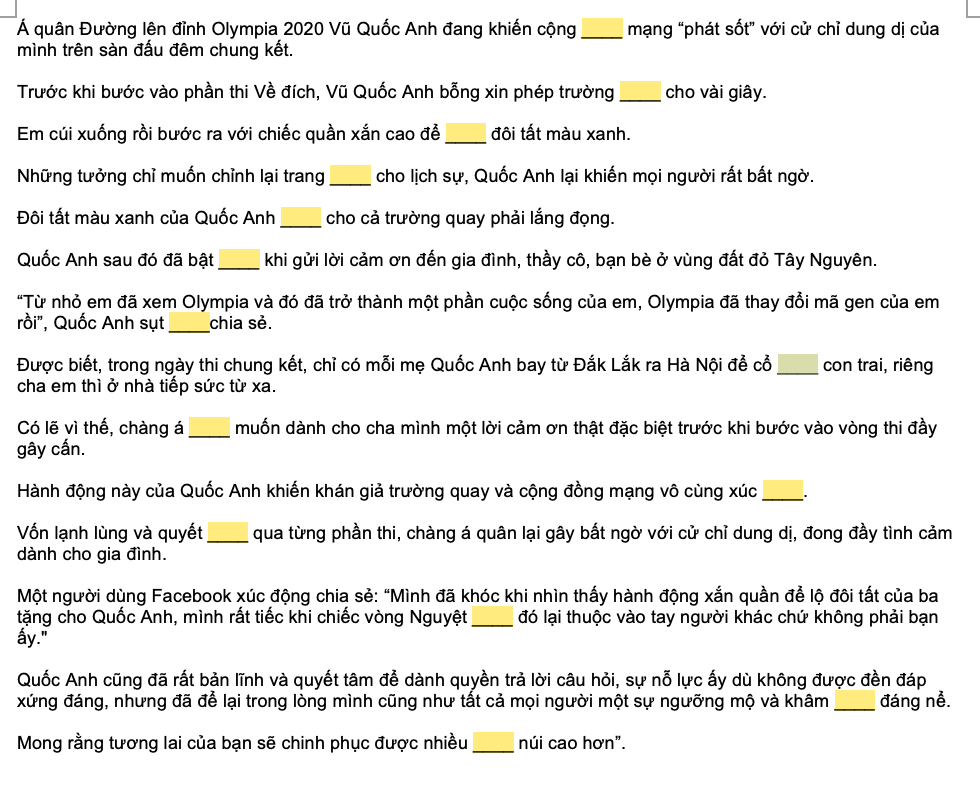
\includegraphics[width=\linewidth]{vicloze} 
\caption{Cloze test for Vietnamese native speakers}
\label{fig:vi-cloze}
\end{center}   
\end{figure}

\subsection{Python script to create stimuli}

\lstinputlisting[language=Python]{createwavsqual.py} 

\subsection{Praat script for acoustic analysis}
\lstinputlisting[language=Python]{get-F0-script.txt} 
\nocite{*}
\bibliographystyle{acm}
\bibliography{CitesforStressPaper.bib}{}

\end{document}